\chapter{Implementation of GNU Taler}\label{chapter:implementation}

This chapter describes the implementation of GNU Taler in detail.  Concrete
design decisions, protocol details and our reference implementation are
discussed.

We implemented the GNU Taler protocol in the context of a payment system for
the web, as shown in Figure~\ref{fig:taler-arch}.  The system was designed for
real-world usage with current web technologies and within existing
financial systems.

The following technical goals and constraints influenced the design of the
concrete protocol and implementation:
\begin{itemize}
  \item The implementation should allow payments in browsers with hardened
    security settings.  In particular, it must be possible to make a payment
    without executing JavaScript on a merchant's website and without having to
    store (session-)cookies or requiring a login.
  \item Cryptographic evidence should be available to all parties in case of a
    dispute.
  \item In addition to the guarantees provided by the GNU Taler protocol, the
    implementation must take care to not introduce additional threats to
    security and privacy.  Features that trade privacy for convenience should
    be clearly communicated to the user, and the user must have the choice to
    deactivate them.  Integration with the web should minimize the potential
    for additional user tracking.
  \item The integration for merchants must be simple.  In particular, merchants
    should not have to write code involving cryptographic operations or have to
    manage Taler-specific secrets in their own application processes.
  \item The web integration must not be specific to a single browser platform, but
    instead must be able to use the lowest common denominator of what is
    currently available.  User experience enhancements supported for only
    specific platforms are possible, but fallbacks must be provided for other
    platforms.
  \item URLs should be clean, user-friendly and must have the expected
    semantics when sharing them with others or revisiting them after a session
    expired.
  \item Multiple currencies must be supported.  Conversion between
    different currencies is out of scope.
  \item The implementation should offer flexibility with regards to what
    context or applications it can be used for.  In particular, the
    implementation must make it possible to provide plugins for different
    underlying banking systems and provide hooks to deal with different
    regulatory requirements.
  \item The implementation must be robust against network failures and crash
    faults, and recover as gracefully as possible from data loss.  Operations
    must be idempotent if possible, e.g., accidentally clicking a payment button twice should
    only result in one payment, and refreshing a page should not lead to
    failures in the payment process.
  \item Authorization should be preferred to authentication.  In particular,
    there should be no situations in which the user must enter confidential
    information on a page that cannot be clearly identified as secure.
  \item No flickering or unnecessary redirects.  To complete a payment, the
    number of request, especially in the user's navigation context, should be
    minimized.
  \item While the implementation should integrate well with browsers, it must
    be possible to request and make payments without a browser.  This makes at
    least part of the implementation completely independent of the extremely
    complex browser standards, and makes Taler usable for machine-to-machine
    payments.
    %\item Backwards compatibility (with what?)
\end{itemize}

We now recapitulate how a GNU Taler payment works, with some more details
specific to the implementation.

By instructing their bank to send money to an exchange, the customer creates a
(non-anonymous) balance, called a \emph{reserve}, at the exchange.  Once the
exchange has received and processed the bank transfer, the customer's
\emph{wallet} automatically \emph{drains} the reserve by withdrawing coins from
it until the reserve is empty.  Withdrawing immediately before a purchase should
be avoided, as it decreases the customer's anonymity set by creating a
correlation between the non-anonymous withdrawal and the spending.

To withdraw coins from the exchange, the customer's wallet authenticates itself
using an Ed25519 private key for the customer's reserve.  The customer must
include the corresponding reserve public key in the payment instruction from
the customer's bank to the exchange's bank that funded their reserve.  With a
bank that directly supports Taler on their online banking website, this process
is streamlined for the user, since the wallet automatically creates the key
pair for the reserve and adds the public key to the payment instruction.


While browsing a merchant's website, the website can signal the wallet to
request a payment from a user. The user is then asked to confirm or reject this
proposal.  If the user accepts, the wallet spends coins with the merchant.  The
merchant deposits coins received from the customer's wallet at the exchange.
Since bank transfers are usually costly, the exchange delays and aggregates
multiple deposits into a bigger wire transfer.  This allows GNU Taler to be
used even for microtransactions of amounts smaller than usually handled by the
underlying banking system.

\begin{figure}
  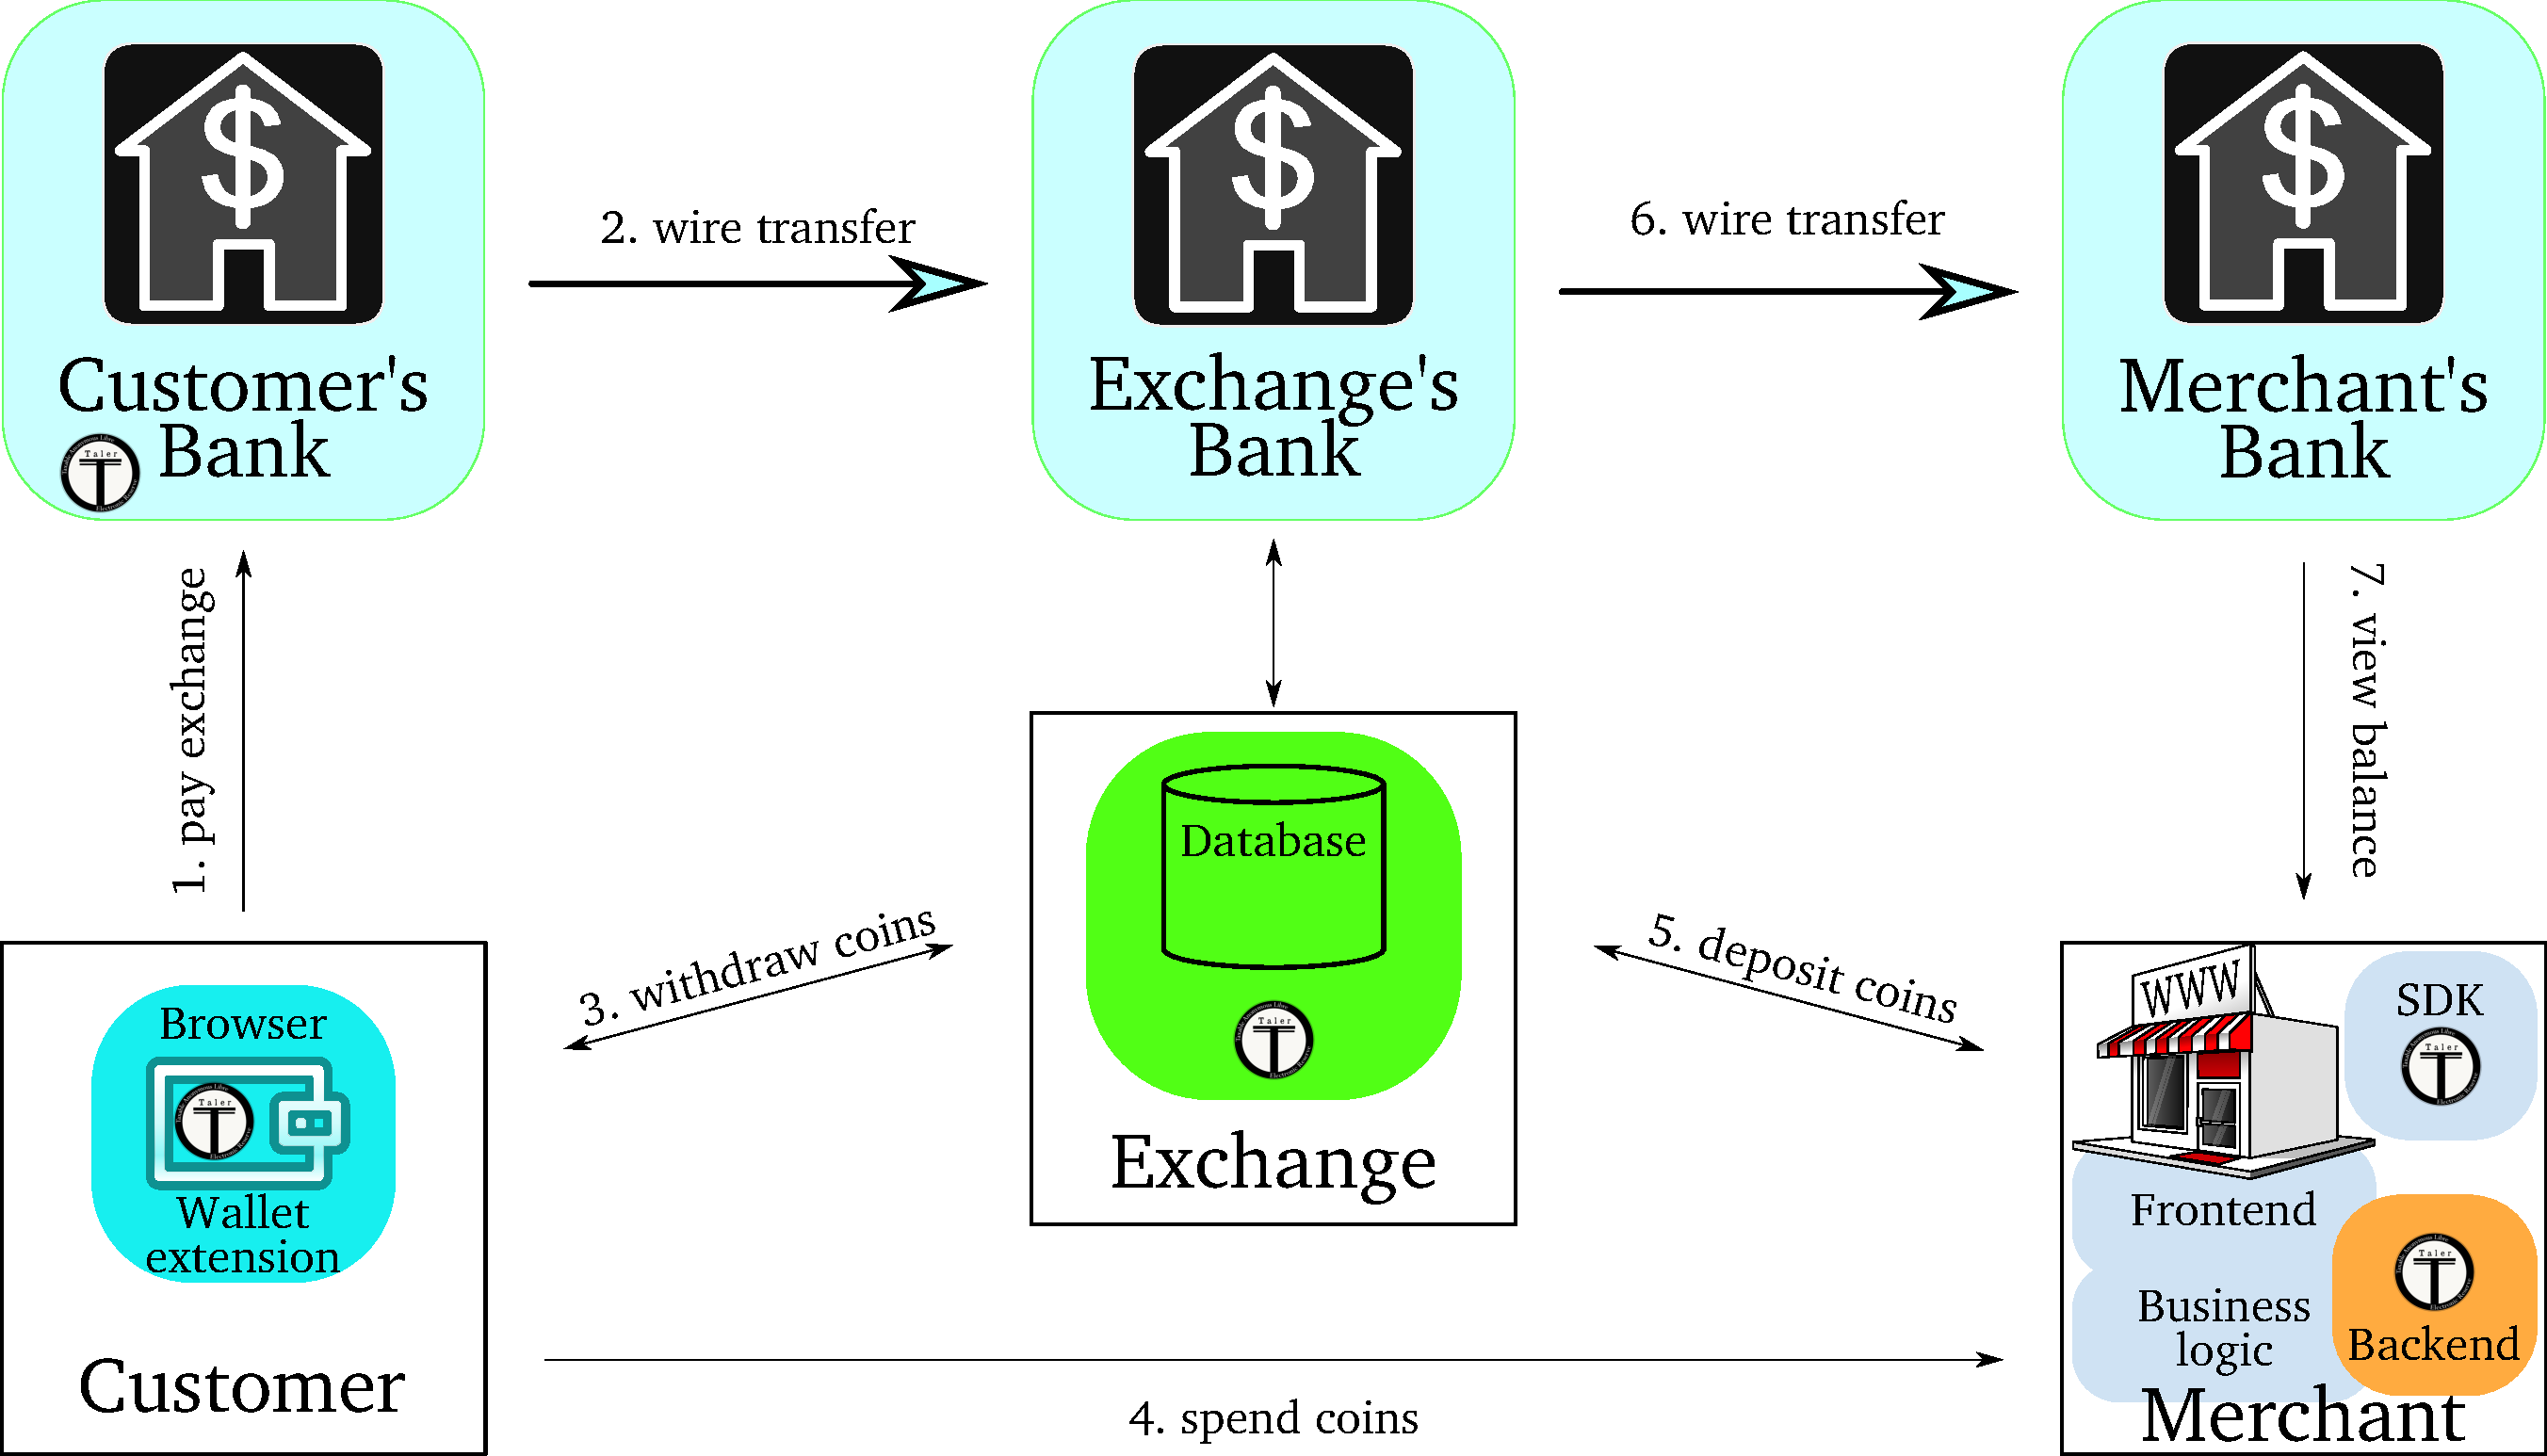
\includegraphics[width=\columnwidth]{taler-arch-full.pdf}
  \caption[Components of GNU Taler in the context of a banking system.]{The different components of the Taler system in the
    context of a banking system providing money creation,
    wire transfers and authentication. (Auditor omitted.)}
  \label{fig:taler-arch-full}
\end{figure}

As shown in Figure~\ref{fig:taler-arch-full}, the merchant is internally split
into multiple components.  The implementation of the Taler protocol and
cryptographic operations is isolated into a separate component, called the
\emph{merchant backend}, which the merchant accesses through an API or software
development kit (SDK) in the programming language of their choice.

Our implementations of the exchange (70,000 LOC) and merchant backend
(20,000 LOC) are written in C using PostgreSQL as the database and
libgcrypt for cryptographic operations.  The \emph{wallet} (10,000
LOC) is implemented in TypeScript as a cross-browser extension using
the WebExtensions API, which is available for a majority of widely
used browsers.  It also uses libgcrypt (compiled to JavaScript) for
cryptographic operations as the required primitives are not yet
natively supported by web browsers.  Sample merchant websites (1,000
LOC) and an example bank (2,000 LOC) with tight Taler integration are
provided in Python.

The code is available at \url{https://git.taler.net/} and a demo
is publicly available at \url{https://demo.taler.net/}.

\section{Overview}

We provide a high-level overview over the implementation,
before discussing the respective components in detail.

\subsection{Taler APIs}
The components of Taler communicate over an HTTP-based, RESTful\footnote{
Some REST purists might disagree, because the Taler APIs do not follow
all REST principles religiously.  In particular, the HATEOAS principle is not followed.
} \cite{fielding2000architectural}
API.  All request payloads and responses are JSON \cite{rfc8259} documents.

Binary data (such as key material, signatures and hashes) is encoded as a
base32-crockford \cite{crockford_base32} string. Base32-crockford is a simple,
case-insensitive encoding of binary data into a subset of the ASCII alphabet
that encodes 5 bits per character.  While this is not the most space-efficient
encoding, it is relatively resilient against human transcription errors.

Financial amounts are treated as fixed-point decimal numbers.  The
implementation internally uses a pair of integers $(v,f)$ with value part $0
\le v \le 2^{52}$ and fractional part $0 \le f < 10^8$ to represent the amount
$a = v + f\cdot 10^{-8}$.  This representation was chosen as the smallest
representable amount is equal to one Satoshi (the smallest representable amount
in Bitcoin), and the largest possible value part (besides being large enough
for typical financial applications) is still accurately representable in 64-bit
IEEE 754 floating point numbers.  These constraints are useful as some
languages such as JavaScript\footnote{Big integers are currently in the process
of being added to the JavaScript language standard.} provide IEEE 753 floating
point numbers as the only numeric type.  More importantly, fixed-point decimal
numbers allow exact representation of decimal values (say \EUR{0.10}), which
is not possible with floating point numbers but essential in financial applications.

Signatures are made over custom binary representations of the respective
values, prefixed with a 64-bit tag consisting of the size of the message (32
bits) and an integer tag (32 bits) uniquely identifying the purpose of the message.
To sign a free-form JSON object, a canonical representation as a string is
created by removing all white space and sorting objects' fields.

In the future, more space-efficient representations (such as BSON\footnote{http://bsonspec.org/} or CBOR \cite{rfc7049})
could be used.  The representation can be negotiated between client and server
in a backwards-compatible way with the HTTP ``Accept'' header.

% signatures!

\subsection{Cryptographic Algorithms}
The following cryptographic primitives are used by Taler:
\begin{itemize}
  \item SHA512 \cite{rfc4634} as a cryptographic hash function
  \item Ed25519 \cite{bernstein2006curve25519} for non-blind signing operations
  \item Curve25519 \cite{bernstein2006curve25519} for the refreshing operation
  \item HKDF \cite{rfc5869} as a key derivation function for the refreshing operation
  \item FDH-RSA blind signatures \cite{bellare2003onemore}
\end{itemize}

We chose these primitives as they are simple, cheap enough and relatively well
studied.  Note that other signature schemes that have the syntax and properties
described in Section~\ref{sec:crypto:instantiation}, such as
\cite{boldyreva2003threshold}, could be used instead of FDH-RSA.  

\subsection{Entities and Public Key Infrastructure}

\begin{figure}
    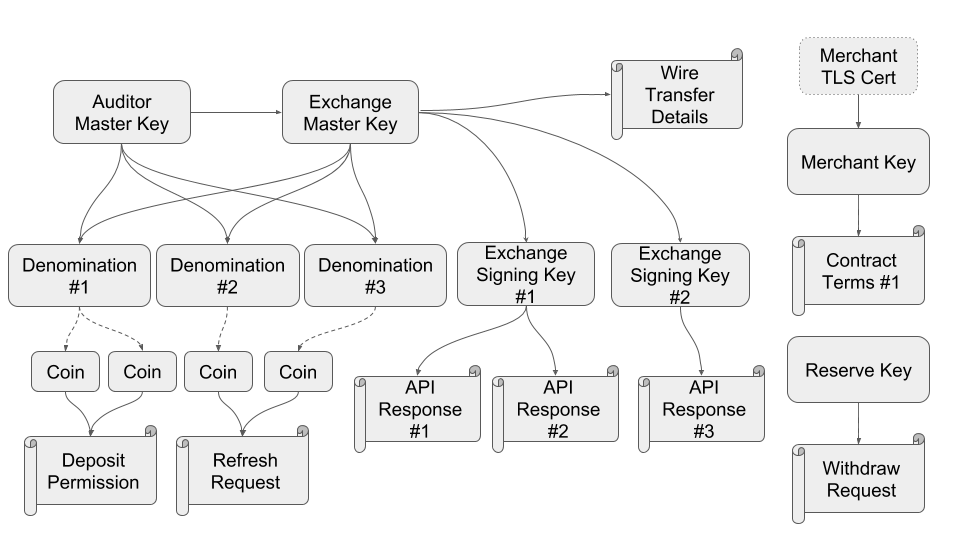
\includegraphics[width=\textwidth]{diagrams/taler-diagram-signatures.png}
    \caption[Entities/PKI in Taler]{Entities/PKI in Taler. Solid arrows denote signatures, dotted arrows denote blind signatures.}
\end{figure}

The public key infrastructure (PKI) used by Taler is orthogonal to the PKI used
by TLS \cite{rfc5246}.  While TLS is used as the transport layer for Taler API
messages, we do not rely on TLS for authenticity or integrity of API queries
and responses.  We do rely on TLS for the confidentiality of digital business
contracts and the authenticity, integrity and confidentiality of digital
product delivery.  For the anonymity properties to hold, the customer must
access the merchant and exchange through an anonymity layer (approximated
by practical implementations like Tor \cite{dingledine2004tor}).

In the case of merchants, we cannot use a trusted auditor or exchange as a
trust anchor, since merchants are not required to register within our PKI to
accept Taler payments.  Here we rely on TLS instead:  The merchant is required
to include their Taler-specific merchant public key in their TLS certificate.
If a merchant fails to do this, the wallet will show a warning when asking the
user to confirm a payment.

\subsubsection{Auditor}
Auditors serve as trust anchors for Taler, and are identified by a single Ed25519 public key.
Wallet implementations come with a pre-defined list of trusted auditors, similar to the certificate
store of browsers or operating systems.

\subsubsection{Exchange}
An exchange is identified by a long term Ed25519 master key and the exchange's
base URL.  The master key is used as an offline signing key, typically stored
on an air-gapped machine.  API requests to the exchange are made by appending
the name of the endpoint to the base URL.

The exchange uses the master key to sign the following data offline:
\begin{itemize}
  \item The exchange's online Ed25519 signing keys.  The online signing keys
    are used to sign API responses from the exchange.  Each signing key has a
    validity period.
  \item The denominations offered by the exchange (explained further in Section~\ref{sec:implementation:denoms}).
  \item The bank accounts supported by the exchange (for withdrawals and deposits) and associated fees.
\end{itemize}

% FIXME: maybe put this later?
The \texttt{<base-url>/keys} HTTP endpoint of the exchange is used by wallets
and merchants to obtain the exchange's signing keys, currently offered
denominations and other details.  In order to reduce traffic, clients can also
request only signing keys and denominations that were created after a specific
time.  The response to \texttt{/keys} is signed by a currently active signing
key, so that customers would have proof in case the exchange gave different sets of
denomination keys to different customers in an attempt to deanonymize them.


\begin{figure}
  \begin{multicols}{2}
  \lstinputlisting[language=C,basicstyle=\ttfamily\tiny,numbers=left]{taler/snippet-keys.txt}
  \end{multicols}
  \caption{Example response for /keys}
\end{figure}


\subsubsection{Coins and Denominations}\label{sec:implementation:denoms}

Denominations are the RSA public keys used to blindly sign coins of a fixed amount, together with information about their
validity and associated fees.  The following information is signed by the exchanges master key for every denomination:
\begin{itemize}
  \item The RSA public key.
  \item The start date, after which coins of this denomination can be withdrawn and deposited.
  \item The withdraw expiration date, after which coins cannot be withdrawn anymore, must be after the start date.
  \item The deposit expiration date, after which coins cannot be deposited anymore, must be after the withdraw expiration date.
  \item The legal expiration date, after which the exchange can delete all records about operations with coins of this denominations,
    must be (typically quite a long time!) after the deposit expiration date.
  \item The fees for a withdraw, deposit, refresh and refund operation with this coin, respectively.
\end{itemize}

\begin{figure}
    \centering
    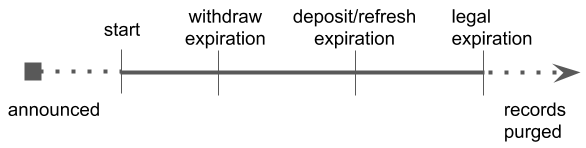
\includegraphics[width=0.7\textwidth]{diagrams/taler-diagram-denom-expiration.png}
    \caption{A denomination's lifetime.}
\end{figure}

An exchange can be audited by zero, one or multiple auditors.  An auditor must
monitor all denominations currently offered by the exchange, and an audit of a
subset of denominations is not intended in the current design.  To allow
customers of an exchange to confirm that it is audited properly, the auditor
signs an auditing request from the exchange, containing basic information about
the exchange as well as all keys offered during the auditing period.  In
addition to the full auditing request, the auditor also signs an individual
certificate for each denomination individually, allowing clients of the
exchange to incrementally verify newly offered denominations.

\subsubsection{Merchant}
The merchant has one Ed25519 key pair that is used to sign responses to the
customer and authenticate some requests to the exchange.  Depending on the
legislation that applies to a particular GNU Taler deployment, merchants might
not need to establish an a priori relationship with the exchange, but instead
send their bank account information during or after the first deposit of a
payment from a customer.

% FIXME: we never write here that the merchant accepts payments from all trusted auditors/exchanges
% automatically
% FIXME: citation for this?
% FIXME: are there jurisdictions where KYC would apply to the exchange's customer?
In some jurisdictions, exchanges are required to follow know-your-customer
(KYC) regulations and to verify the identity of merchants \cite{arner2018identity} using that particular
exchange for deposits.  Typically, the identity of a merchant only has to be
verified if a merchant exceeds a certain threshold of transactions in a given
time span.  As the KYC registration process can be costly to the exchange, this
requirement is somewhat at odds with merchants accepting payments from all
exchanges audited by a trusted auditor, since KYC registration needs to be done
at every exchange separately.  It is, however, unavoidable to run a legally
compliant payment system.

A merchant is typically configured with a set of trusted auditors and
exchanges, and consequently accepts payments with coins of denominations from a
trusted exchange and denominations audited by a trusted auditor.

In order to make the deployment of Taler easier and more secure, the parts that
deal with the merchant's private key and cryptographic operations are isolated
into a separate service (the merchant backend) with a well-defined RESTful HTTP API.
This concept is similar to payment gateways used commonly for credit card
payments.  The merchant backend can be deployed on-premise by the online shop,
or run by a third party provider that is fully trusted by the merchant.

\subsubsection{Bank}
Since the banks are third parties that are not directly part of Taler, they do
not participate directly in Taler's PKI.

\subsubsection{Customer}
Customers are not registered with an exchange, instead they use the private
keys of reserves that they own to authenticate with the exchange.  The exchange
knows the reserve's public key from the subject/instruction data of the wire
transfer.  Wire transfers that do not contain a valid public key are
automatically reversed.


\subsection{Payments}

\newlength{\maxheight}
\setlength{\maxheight}{\heightof{\small W}}
\newcommand{\bffmt}[1]{%
  \footnotesize
  \centering
  \raisebox{0pt}[\maxheight][0pt]{#1}%
}

\begin{figure}
\centering
\begin{bytefield}[bitwidth=0.2em,bitheight=3ex,boxformatting=\bffmt]{128}
  \bitheader{0,31,63,95,127} \\
  \bitbox{32}{size} & \bitbox{32}{purpose} & \bitbox{64}{timestamp} \\
  \wordbox{2}{merchant public key} \\
  \wordbox{4}{contract terms hash} \\
  \bitbox{64}{deposit deadline} & \bitbox{64}{refund deadline} \\
  \wordbox{4}{KYC / account info hash}
\end{bytefield}
\caption{The contract header that is signed by the merchant.}
\end{figure}

\begin{figure}
\centering
\begin{bytefield}[bitwidth=0.2em,bitheight=3ex,boxformatting=\bffmt]{128}
  \bitheader{0,31,63,95,127} \\
  \bitbox{32}{size} & \bitbox{32}{purpose} & \bitbox{64}{timestamp} \\
  \wordbox{4}{contract header hash} \\
  \wordbox{2}{coin public key} \\
  \bitbox[lrt]{128}{contributed amount} \\
  \bitbox[lrb]{64}{} & \bitbox[ltr]{64}{} \\
  \bitbox[lrb]{128}{deposit fee} \\
\end{bytefield}
\caption{The deposit permission signed by the customer's wallet.}
\end{figure}


Payments in Taler are based on \emph{contract terms}, a JSON object that
describes the subject and modalities of a business transaction.  The
cryptographic hash of such a contract terms object can be used as a globally
unique identifier for the business transaction.  Merchants must sign the
contract terms before sending them to the customer, allowing a customer to
prove in case of a dispute the obligations of the merchant resulting from the
payment.

Unless a third party needs to get involved in a dispute, it is sufficient (and
desirable for data minimization) that only the merchant and the customer know
the full content of the contract terms.  The exchange, however,  must still
know the parts of the contract terms that specify payment modalities, such as
the refund policy, micropayment aggregation deadline and the merchant's KYC
registration data (typically a hash to prove the KYC enrollment of the
merchant).

Thus, the merchant's signature is made over the \emph{contract header},
which contains the contract terms hash, as well as the payment modalities.

In addition to the data provided by the merchant, the contract terms contain a
\emph{claim\_pub} field whose value is provided by the customer.
This field is an Ed25519 public key, and the customer can use the corresponding
private key to prove that they have indeed obtained the individual contract
terms from the merchant, and did not copy contract terms that the merchant gave
to another customer.  Note that this key is not a permanent identity of the
customer, but should be freshly generated for each payment.

The signed contract header is created by the merchant's backend from an
\emph{order}, which is the ``blueprint'' for the contract terms.  The order is
generated by the merchant's frontend and contains a subset of the data
contained in the contract terms.  Missing data (in particular the merchant's
bank account information, public key and accepted auditors/exchanges) and
the claim public key obtained from the customer is automatically added by the merchant
backend.  This allows applications to process payments without having to
specify Taler-internal details.  In fact, the smallest possible order only
needs to contain two fields:  the amount to be paid and a human-readable
summary of the payment's subject.

An order contains an \emph{order ID}, which is an identifier that is unique
within a given merchant and can be a human-friendly identifier such as a
booking number.  If the order ID is not manually provided, it is automatically
filled in by the merchant backend.  It can be used to refer to the payment
associated with the order without knowing the contract terms hash, which is
only available once the customer has provided their claim public key.

To initiate a payment, the merchant sends the customer an \emph{unclaimed}
contract terms URL.  The customer can download and thereby claim ownership of
the contract by appending their claim public key $p$ as a query parameter to the unclaimed
contract terms URL and making an HTTP \texttt{GET} request to the resulting URL.
The customer must then verify that the resulting contract terms are signed
correctly by the merchant and that the contract terms contain their claim public key $p$.
A malicious customer could try to claim other customers' contracts by guessing
contract term URLs and appending their own claim public key.  For products that have
limited availability, the unclaimed contract URL must have enough entropy so
that malicious customers are not able to guess them and claim them before the
honest customer.\footnote{Note that this URL cannot be protected by a session
cookie, as it might be requested from a different session context than the
user's browser, namely in the wallet.}

% FIXME: put this in a sidebox?
To give an example, an online shop for concert tickets might allow users to put
themselves on a waiting list, and will send them an email once a ticket
becomes available.  The contract terms URL that allows the customer to purchase
the ticket (once they have visited a link in this email), should contain an
unguessable nonce, as otherwise an attacker might be able to predict the URL
and claim the contract for the concert ticket before the customer's wallet can.

In order to settle the payment, the customer must sign a \emph{deposit
permission} for each coin that comprises the payment.  The deposit permission
is a message signed by the coin's private key, containing
\begin{itemize}
  \item the amount contributed by this coin to the payment,
  \item the merchant's public key
  \item the contract header together with the merchant's signature on it,
  \item the time at which the deposit permission was signed.
\end{itemize}

After constructing the deposit permissions for a contract, the customer sends
them to the merchant by doing an HTTP \texttt{POST} request to the
\texttt{pay\_url} indicated by the merchant in the contract terms.  The
merchant individually \emph{deposits} each deposit permission with the
exchange.

The merchant responds with a payment confirmation to the customer after it has
successfully deposited the customer's coins with the exchange.  The payment
confirmation can be used by the customer to prove that they completed the
payment before the payment deadline indicated in the contract terms.

Note that the depositing multiple coins with the exchange deliberately does not
have transactional semantics.  Instead, each coin is deposited in an individual
transaction.  This allows the exchange to be horizontally scaled (as discussed
in Section~\ref{sec:implementation-improvements}) more easily, as deposit
transaction might otherwise have to span multiple database shards.

The lack of transactional semantics, however, means that it must be possible to
recover from partially completed payments.  There are several cases: If one of
the coins that the customer submitted as payment to the merchant is invalid
(e.g., because the wallet's state was restored from a backup), the customer can
re-try the partially completed payment and provide a different coin instead.
If that is not possible or desired by the customer, the merchant may voluntarily give a
refund on the coins that have been previously deposited.  The reference
implementation of the merchant backend offers refunds for partially completed
payments automatically.

% FIXME: explain why!
If refunds were disabled for the payment, the merchant does not cooperate in
giving refunds for a partially completed payment, or becomes unresponsive after
partially depositing the customer's coin, the customer has two options: They
can either complete the deposits on the merchant's behalf, and then use the
deposit permissions to prove (either to the merchant or to a court) that they
completed the payment.

% FIXME: put this in info box?
Another possibility would be to allow customers to request refunds for partially
completed payments themselves, directly from the exchange.
This requires that the merchant additionally
includes the amount to be paid for the contract in the contract header, as the
exchange needs to know that amount to decide if a payment with multiple coins
is complete.  We do not implement this approach, since it implies that the
exchange always learns the exact prices of products that the merchant sells, as
opposed to just the merchant's total revenue.

The customer could also reveal the contract terms to the exchange to prove that
a payment is incomplete, but this is undesirable for privacy reasons, as the
exchange should not learn about the full details of the business agreement
between customer and merchant.

\subsection{Resource-based Web Payments}
In order to integrate natively with the concepts and architecture of the web,
Taler supports paying for a web resource in the form of a URL.  In fact all
Taler contract terms contain a \emph{fulfillment URL}, which identifies the
resource that is being paid for.  If the customer is not paying for a digital
product (such as an movie, song or article), the fulfillment URL can point to a
confirmation page that shows further information, such as a receipt for a
donation or shipment tracking information for a physical purchase.  A
fulfillment URL does not necessarily refer to a single item, but could also
represent a collection such as a shopping basket.

The following steps illustrate a typical payment with the online shop
\nolinkurl{alice-shop.example.com}.

\newcommand{\contl}[0]{\mbox{\textcolor{blue}{$\hookrightarrow$}\space}}

\lstdefinelanguage{none}{
  identifierstyle=
}
\lstdefinestyle{myhttp}{
  breaklines=true,
  breakindent=3em,
  escapechar=*,
  postbreak=\contl,
  basicstyle=\ttfamily,
  showspaces=true,
}

\begin{enumerate}
  \item The user opens the shop's page and navigates to a paid resource, such
    as \nolinkurl{https://alice-shop.example.com/essay-24.pdf}.
  \item The shop sends a response with HTTP status ``402 Payment Required''
    with the headers (\contl marks a continued line)
\begin{lstlisting}[style=myhttp]
Taler-Contract-Url: https://alice-shop.example.com/*\break\contl*contract?product=essay-24.pdf
Taler-Resource-Url: https://alice-shop.example.com/*\break\contl*essay-24.pdf
\end{lstlisting}
  \item Since the user's wallet does not yet contain contract terms with the
    fulfillment URL \nolinkurl{https://alice-shop.example.com/esasy-24.pdf}
    that matches the resources URL, it claims the contract by generating a
    claim key pair $(s, p)$  and requesting the contract URL with the claim
    public key $p$ as additional parameter:
    \nolinkurl{https://alice-shop.example.com/contract?product=essay-24.pdf\&claim_pub=}$p$.
  \item The wallet displays the contract terms to the customer and asks them to
    accept or decline.  If the customer accepted the contract, the wallet sends
    a payment to the merchant.  After the merchant received a valid payment,
    it marks the corresponding order as paid.
  \item The wallet constructs the extended fulfillment URL by adding the order
    id from the contract as an additional parameter and navigates the browser
    to the resulting URL
    \nolinkurl{https://alice-shop.example.com/esasy-24.pdf?order\_id=...}.
  \item The shop receives the request to the extended fulfillment URL and
    checks if the payment corresponding to the order ID was completed.  In case
    the payment was successful, it serves the purchased content.
\end{enumerate}

To avoid checking the status of the payment every time, the merchant can
instead set a session cookie (signed/encrypted by the merchant) in the user's
browser which indicates that \texttt{essay-24.pdf} has been purchased.

The resource-based payment mechanism must also handle the situation where a
customer navigates again to a resource that they already paid for, without
directly navigating to the extended fulfillment URL.  In case no session cookie
was set for the purchase or the cookie was deleted / has expired, the customer would
be prompted for a payment again.  To avoid this, the wallet tries to find an
existing contract whose plain fulfillment URL matches the resource URL
specified in the merchant's HTTP 402 response.  If such an existing payment was
found, the wallet instead redirects the user to the extended fulfillment URL
for this contract, instead of downloading the new contract terms and prompting
for payment.

In the example given above, the URL that triggers the payment is the same as the fulfillment URL.
This may not always the case in practice.  When the merchant backend is hosted by a third
party, say \nolinkurl{https://bob.example.com/}, the page that triggers the payment
even has a different origin, i.e., the scheme, host or port may differ \cite{rfc6454}.

This cross-origin operation presents a potential privacy risk if not
implemented carefully.
To check whether a user has already paid for a particular
resource with URL $u$, an arbitrary website could send an HTTP 402 response with
the ``Taler-Resource-Url'' header set to $u$ and the ``Taler-Contract-Url''
set to a URL pointing to the attacker's server.  If the user paid for $u$, the
wallet will navigate to the extended fulfillment URL corresponding to $u$.
Otherwise, the wallet will try to download a contract from the URL given by the
attacker.  In order to prevent this attack on privacy, the wallet must only
redirect to $u$ if the origin of the page responding with HTTP 402 is the same
origin as either the $u$ or the pay URL.\footnote{This type of countermeasure is well
known in browsers as the same origin policy, as also outlined in \cite{rfc6454}.}

\subsubsection{Loose Browser Integration}\label{sec:loose-browser-integration}

The payment process we just described does not directly work in browsers that do not
have native Taler integration, as the browser (or at least a browser extension)
would have to handle the HTTP status code 402 and handle the Taler-specific headers correctly.
We now define a fallback, which is transparently implemented in the reference merchant backend.

In addition to indicating that a payment is required for a resource in the HTTP status code and header,
the merchant includes a fallback URL in the body of the ``402 Payment Required'' response.  This URL must have the custom URL scheme
\texttt{taler}, and contains the contract terms URL (and other Taler-specific settings normally specified in headers)
as parameters.  The above payment would include a link (labled, e.g., ``Pay with GNU Taler'') to the following URL, encoding
the same information as the headers:
\begin{lstlisting}[style=myhttp]
taler:pay?*\break\contl*contract_url=*\break\contl*https%3A%2F%2Falice-shop.example.com%2Fcontract%3Fproduct%3Dessay-24.pdf*\break\contl*&resource_url=*\break\contl*https%3A%2F%2Falice-shop.example.com%2Fessay-24.pdf
\end{lstlisting}

This fallback can be disabled for requests from user agents that are known to
natively support GNU Taler.

GNU Taler wallet applications register themselves as a handler for the
\texttt{taler} URI scheme, and thus following a \texttt{taler:pay} link opens
the dedicated wallet, even if GNU Taler is not supported by the browser or a
browser extension.  Registration a custom protocol handler for a URI scheme is
possible on all modern platforms with web browsers that we are aware of.

Note that wallets communicating with the merchant do so from a different
browsing context, and thus the merchant backend cannot rely on cookies that
were set in the customer's browser when using the shop page.

We chose HTTP headers as the primary means of signaling to the wallet (instead
of relying on, e.g., a new content media type), as it allows the fallback content
to be an HTML page that can be rendered by all browsers. Furthermore,
current browser extension mechanism allow intercepting headers synchronously
before the rendering of the page is started, avoiding visible flickering caused by
intermediate page loads.

\subsection{Session-bound Payments and Sharing}
As we described the payment protocol so far, an extended fulfillment URL
is
not bound to a browser session.  When sharing an extended fulfillment
URL, another user would get access to the same content.  This might be appropriate
for some types of fulfillment pages (such as a donation receipt), but is generally not
appropriate when digital content is sold.  Even though it is trivial to share digital content
unless digital restrictions management (DRM) is employed, the ability to share
links might set the bar for sharing too low.

While the validity of a fulfillment URL could be limited to a certain time,
browser session or IP address, this would be too restrictive for scenarios where
the user wants to purchase permanent access to the content.

As a compromise, Taler provides \emph{session-bound} payments.  For
session-bound payments, the seller's website assigns the user a random session
ID, for example, via a session cookie.  The extended fulfillment URL for
session-bound payments is constructed by additionally specifying the URL
parameter \texttt{session\_sig}, which contains proof that the user completed
(or re-played) the payment under their current session ID.

To initiate a session-bound payment, the HTTP 402 response must additionally
contain the ``Taler-Session-Id'' header, which will cause the wallet to
additionally obtain a signature on the session ID from the merchant's pay URL,
by additionally sending the session ID when executing (or re-playing) the
payment.
As an optimization, instead of re-playing the full payment, the wallet can also
send the session ID together with the payment receipt it obtained from the
completed payment with different session ID.

Before serving paid content to the user, the merchant simply checks if the
session signature matches the assigned session and contract terms.  To simplify
the implementation of the frontend, this signature check can be implemented as
a request to the GNU Taler backend.  Using session signatures instead of storing
all completed session-bound payments in the merchant's database saves storage.

While the coins used for the payment or the payment receipt could be shared
with other wallets, it is a higher barrier than just sharing a URL.  Furthermore, the
merchant could restrict the rate at which new sessions can be created for the
same contract terms and restrict a session to one IP address, limiting sharing.

For the situation where a user accesses a session-bound paid resource and
neither has a corresponding contract in their wallet nor does the merchant
provide a contract URL to buy access to the resource, the merchant can specify
an \emph{offer URL} in the ``Taler-Offer-Url'' header.  If the wallet is not
able to take any other steps to complete the payment, it will redirect the user
to the offer URL.  As the name suggests, the offer URL can point to a page with
alternative offers for the resource, or some other explanation as to why the
resource is not available anymore.

\subsection{Embedded Content}
So far we only considered paying for a single, top-level resource,
namely the fulfillment URL.  In practice, however, websites are composed of
many subresources such as embedded images and videos.

We describe two techniques to ``paywall'' subresources behind a GNU Taler
payment.  Many other approaches and variations are possible.
\begin{enumerate}
  \item Visiting the fulfillment URL can set a session cookie.  When a
    subresource is requested, the server will check that the customer has the
    correct session cookie set.
  \item When serving the fulfillment page, the merchant can add an additional
    authentication token to the URLs of subresources.  When the subresource is
    requested, the validity of the authentication token is checked.  If the
    merchant itself (instead of a Content Delivery Network that supports token
    authentication) is serving the paid subresource, the order ID and session
    signature can also be used as the authentication token.
\end{enumerate}

It would technically be possible to allow contract terms to refer to multiple
resources that are being purchased by including a list or pattern that defines
a set of URLs.  The browser would then automatically include information to
identify the completed payment in the request for the subresource.  We
deliberately do not implement this approach, as it would require deeper
integration in the browser than possible on many platforms.  If not restricted
carefully, this feature could also be used as an additional method to track the
user across the merchant's website.

\subsection{Contract Terms}
The contract terms, only seen by the customer and the merchant (except when a tax audit of the merchant is requested)
contain the following information:
\begin{itemize}
  \item The total amount to be paid,
  \item the \texttt{pay\_url}, an HTTP endpoint that receives the payment,
  \item the deadline until the merchant accepts the payment (repeated in the signed contract header),
  \item the deadline for refunds (repeated in the signed contract header),
  \item the claim public key provided by the customer, used to prove they have claimed the contract terms,
  \item the order ID, which is a short, human-friendly identifier for the contract terms within
    the merchant,
  \item the \texttt{fulfillment\_url}, which identifies the resources that is being paid for,
  \item a human-readable summary and product list,
  \item the fees covered by the merchant (if the fees for the payment exceed this value, the
    customer must explicitly pay the additional fees),
  \item depending on the underlying payment system, KYC registration information
    or other payment-related data that needs to be passed on to the exchange (repeated in the signed contract header),
  \item the list of exchanges and auditors that the merchants accepts for the payment,
  \item information about the merchant, including the merchant public key and contact information.
\end{itemize}


\subsection{Refunds}
By signing a \emph{refund permission}, the merchant can ``undo'' a deposit on a
coin, either fully or partially.  The customer can then spend (or refresh) the
refunded value of the coin again.  A refund is only possible before the refund
deadline (specified in the contract header).  After the refund deadline has
passed (and before the deposit deadline) the exchange makes a bank transfer the
merchant with the aggregated value from deposits, a refund after this point
would require a bank transfer back from the merchant to the exchange.

Each individual refund on each coin incurs fees; the
refund fee is subtracted from the amount given back to the customer and kept by
the exchange.

Typically a refund serves either one of the following purposes:
\begin{itemize}
  \item An automatic refund is given to the customer when a payment only
    partially succeeded.  This can happen when a customer's wallet accidentally
    double-spends, which is possible even with non-malicious customers and caused by data
    loss or delayed/failed synchronization between the same user's wallet on
    multiple devices.  In these cases, the user can choose to re-try the
    payment with different, unspent coins (if available) or to ask for a refund
    from the merchant.
  \item A voluntary refund can be given at the discretion of the merchant,
    for example, when the customer is not happy with their purchase.
\end{itemize}
Refunds require a signature by the merchant, but no consent from the customer.

A customer is notified of a refund with the HTTP 402 Payment Required status
code and the ``Taler-Refund'' header.  The value of the refund header is a
URL. An HTTP \texttt{GET} request on that URL will return a list of refund confirmations that the
merchant received from the exchange.

\subsection{Tipping}
Tipping in Taler uses the ``withdraw loophole'' (see \ref{taler:design:tipping}) to allow the
merchant\footnote{We still use the term ``merchant'', since donations use the same software component
as the merchant, but ``donor'' would be more accurate.} to donate small amounts (without any associated contract terms or legal
obligations) into the user's wallet.

To be able to give tips, the merchant must create a reserve with an exchange.  The reserve private key
is used to sign blinded coins generated by the user that is being given the tip.

The merchant triggers the wallet by returning an HTTP 402 Payment Required
response that includes the ``Taler-Tip'' header. The value of the tip header (called the
tip token) contains
\begin{itemize}
  \item the amount of the tip,
  \item the exchange to use,
  \item a URL to redirect after processing the tip,
  \item a deadline for picking up the tip,
  \item a merchant-internal unique ID for the tip, and
  \item the \emph{pickup URL} for the tip.
\end{itemize}
Upon receiving the tip token, the wallet creates coin planchets that sum up to at most
the amount specified in the tip token, with denominations offered by the exchange specified in the tip token.

The list of planchets is then sent to the merchant via an HTTP \texttt{POST}
request to the tip-pickup URL.  The merchant creates a withdrawal confirmation
signature for each planchet, using the private key of the tipping reserve, and
responds to the HTTP \texttt{POST} request with the resulting list of
signatures.  The user then uses these signatures in the normal withdrawal
protocol with the exchange to obtain coins ``paid for'' by the merchant, but
anonymized and only spendable by the customer.


\section{Bank Integration}
In order to use Taler for real-world payments, it must be integrated with the
existing banking system.  Banks can choose to tightly integrate with Taler and
offer the ability to withdraw coins on their website.  Even existing banks can
be used to withdraw coins via a manual bank transfer to the exchange, with the
only requirement that the 52 character alphanumeric, case-insensitive encoding
of the reserve public key can be included in the transaction without
modification other than case folding and white space
normalization.\footnote{Some banking systems specify that the subject of the
can be changed, and provide an additional machine-readable ``instruction''
field.  }

\subsection{Wire Method Identifiers}\label{implementation:wire-method-identifiers}
We introduce a new URI scheme \texttt{payto}, which is used in Taler to
identify target accounts across a wide variety of payment systems with uniform
syntax.

In in its simplest form, a \texttt{payto} URI identifies one account of a particular payment system:

\begin{center}
  \texttt{'payto://' TYPE '/' ACCOUNT }
\end{center}

When opening a \texttt{payto} URI, the default action is to open an application
that can handle payments with the given type of payment system, with the target
account pre-filled.  In its extended form, a \texttt{payto} URL can also specify
additional information for a payment in the query parameters of the URI.

In the generic syntax for URIs, the payment system type corresponds to the
authority, the account corresponds to the path, and additional parameters for
the payment correspond to the query parameters.  Conforming to the generic URI
syntax makes parsing of \texttt{payto} URIs trivial with existing parsers.

Formally, a \texttt{payto} URI is an encoding of a partially filled out pro
forma invoice.  The full specification of the \texttt{payto} URI is RFC XXXX. % FIXME!

In the implementation of Taler, \texttt{payto} URIs are used in various places:
\begin{enumerate}
  \item The exchange lists the different ways it can accept money as \texttt{payto} URIs.
    If the exchange uses payment methods that do not have tight Taler integration.
  \item In order to withdraw money from an exchange that uses a bank account type that
    does not typically have tight Taler integration, the wallet can generate a link and a QR code
    that already contains the reserve public key.  When scanning the QR code with a mobile device that
    has an appropriate banking app installed, a bank transfer form can be pre-filled and the user only has to confirm the
    transfer to the exchange.
  \item The merchant specifies the account it wishes to be paid on as a \texttt{payto} URI, both in
    the configuration of the merchant backend as well as in communication with the exchange.
\end{enumerate}

A major advantage of encoding payment targets as URIs is that URI schemes can be registered
with an application on most platforms, and will be ``clickable'' in most applications and open the right
application when scanned as a QR code.  This is especially useful for the first use case listed above; the other use cases
could be covered by defining a media type instead \cite{rfc6838}.

% FIXME: put into side box
As an example, the following QR code would open a banking application that supports SEPA payments,
pre-filled with a 15\EUR{} donation to the bank account of GNUnet:

\begin{center}
\qrcode[hyperlink,height=5em]{payto://sepa/DE67830654080004822650?amount=EUR:15}
\end{center}

\subsection{Demo Bank}
For demonstration purposes and integration testing, we use our toy bank
implementation\footnote{\url{https://git.taler.net/bank.git}}, which might be
used in the future for regional currencies or accounting systems (e.g., for a
company cafeteria).  The payment type identifier is \texttt{taler-bank}.  The
authority part encodes the base URL of the bank, and the path must be the
decimal representation of a single integer between $1$ and $2^{52}$, denoting
the internal demo bank account number.

\subsection{EBICS and SEPA}
The Electronic Banking Internet Communication Standard\footnote{\url{http://www.ebics.org}} (EBICS) is a standard
for communicating with banks, and is widely used in Germany, France and
Switzerland, which are part of the Single European Payment Area (SEPA).  EBICS
itself is just a container format.  A commonly supported payload for EBICS is
ISO 2022, which defines messages for banking-related business processes.

Integration of GNU Taler with EBICS is currently under development, and would
allow Taler to be easily deployed in many European countries, provided that the
exchange provider can obtain the required banking license.

\subsection{Blockchain Integration}
Blockchains such as Bitcoin could also be used as the underlying financial
system for GNU Taler, provided that merchants and customers trust the exchange to be honest.

With blockchains that allow more complex smart contracts, the auditing
functionality could be implemented by the blockchain itself.  In particular,
the exchange can be incentivized to operate correctly by requiring an initial
safety deposit to the auditing smart contract, which is distributed to
defrauded participants if misbehavior of the exchange is detected.

\section{Exchange}

\begin{figure}
    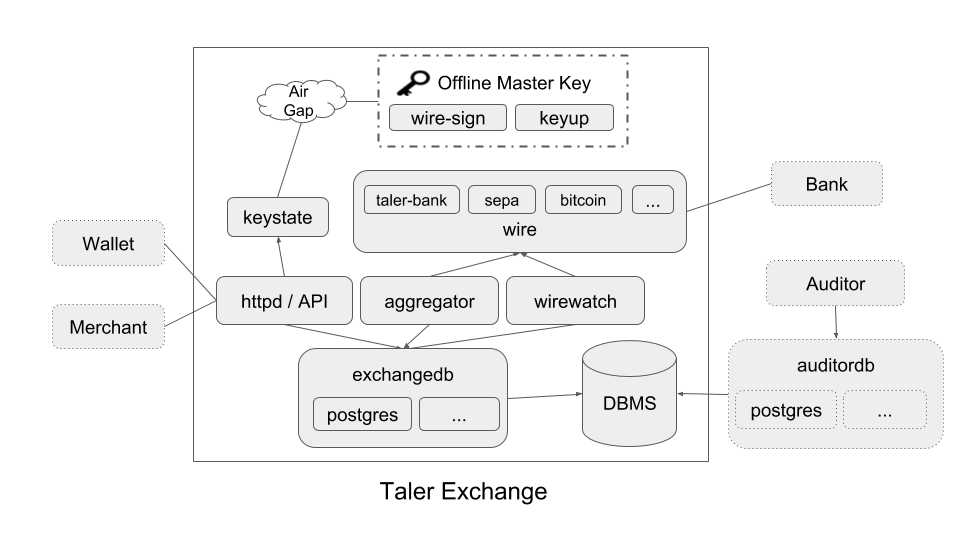
\includegraphics[width=\textwidth]{diagrams/taler-diagram-exchange.png}
    \caption{Architecture of the exchange reference implementation}
\end{figure}

The exchange consists of three independent processes:
\begin{itemize}
  \item The \texttt{taler-exchange-httpd} process handles HTTP requests from clients,
  mainly merchants and wallets.
  \item The \texttt{taler-exchange-wirewatch} process watches for wire transfers
  to the exchange's bank account and updates reserves based on that.
  \item The \texttt{taler-exchange-aggregator} process aggregates outgoing transactions
  to merchants.
\end{itemize}
All three processes exchange data via the same database.  Only
\texttt{taler-exchange-httpd} needs access to the exchanges online signing keys
and denomination keys.

The database is accessed via a Taler-specific database abstraction layer.
Different databases can be supported via plugins; at the time of writing this,
only a PostgreSQL plugin has been implemented.

Wire plugins are used as an abstraction to access the account layer that Taler
runs on.  Specifically, the \textit{wirewatch} process uses the plugin to monitor
incoming transfers, and the aggregator process uses the wire plugin to make
wire transfers to merchants.

The following APIs are offered by the exchange:
\begin{description}
  \item[Announcing keys, bank accounts and other public information]  The
    exchange offers the list of denomination keys, signing keys, auditors,
    supported bank accounts, revoked keys and other general information needed
    to use the exchange's services via the \texttt{/keys} and \texttt{/wire}
    APIs.
  \item[Obtaining entropy] As we cannot be sure that all client-devices have
    an adequate random number generator, the exchange offers the \texttt{/seed}
    endpoint to download some high-entropy value.  Clients should mix this
    seed with their own, locally-generated entropy into an entropy pool.
  \item[Reserve status and withdrawal] After having wired money to the exchange,
    the status of the reserve can be checked via the \texttt{/reserve/\$RESERVE\_PUB/status} API.  Since
    the wire transfer usually takes some time to arrive at the exchange, wallets should periodically
    poll this API, and initiate a withdrawal with \texttt{/reserve/\$RESERVE\_PUB/withdraw} once the exchange received the funds.
  \item[Deposits and tracking]  Merchants transmit deposit permissions they have received from customers
    to the exchange via the \texttt{/coins/\$COIN\_PUB/deposit} API.  Since multiple deposits are aggregated into one wire transfer,
    the merchant additionally can use the exchange's \texttt{/transfers/\$WTID} API that returns the list of deposits for a wire transfer
    identifier (WTID) included in the wire transfer to the merchant, as well as the \texttt{/deposits/\$H\_WIRE/\$MERCHANT\_PUB/\$H\_CONTRACT\_TERMS/\$COIN\_PUB} API to look up
    which wire transfer included the payment for a given deposit.
  \item[Refresh] Refreshing consists of two stages. First, using \texttt{/coins/\$COIN\_PUB/melt} an old, possibly dirty coin is melted and thus devaluted. The committment made by the wallet during the melt and the resulting $\gamma$-challenge from the exchange are associated with a {\em refresh session}.  Then, using \texttt{/refreshes/\$RCH/reveal} the wallet can answer the challenge and obtain fresh coins as change.  Finally, \texttt{/coins/\$COIN\_PUB/link} provides the link deterrent against refresh abuse.
  \item[Refunds] The refund API (\texttt{/coins/\$COIN\_PUB/refund}) can ``undo'' a deposit if the merchant gave their signature, and the aggregation deadline
    for the payment has not occurred yet.
  \item[Recoup]  The recoup API (\texttt{/coins/\$COIN\_PUB/recoup}) allows customers to be compensated
    for coins whose denomination key has been revoked.  Customers must send either a full withdrawal transcript that
    includes their private blinding factor, or a refresh transcript (of a refresh that had the revoked denominations as one of the targets)
    that includes blinding factors.  In the former case, the reserve is credited, in the latter case, the source coin of the
    refresh is refunded and can be refreshed again.
\end{description}

New denomination and signing keys are generated and signed with the exchange's master
secret key using the \texttt{taler-exchange-keyup} utility, according to a key schedule
defined in the exchange's configuration.  This process should be done on an air-gapped
offline machine that has access to the exchange's master signing key.

Generating new keys with \texttt{taler-exchange-keyup} also generates an
auditing request file, which the exchange should send its auditors.  The auditors then
certify these keys with the \texttt{taler-auditor-sign} tool.

\begin{figure}
    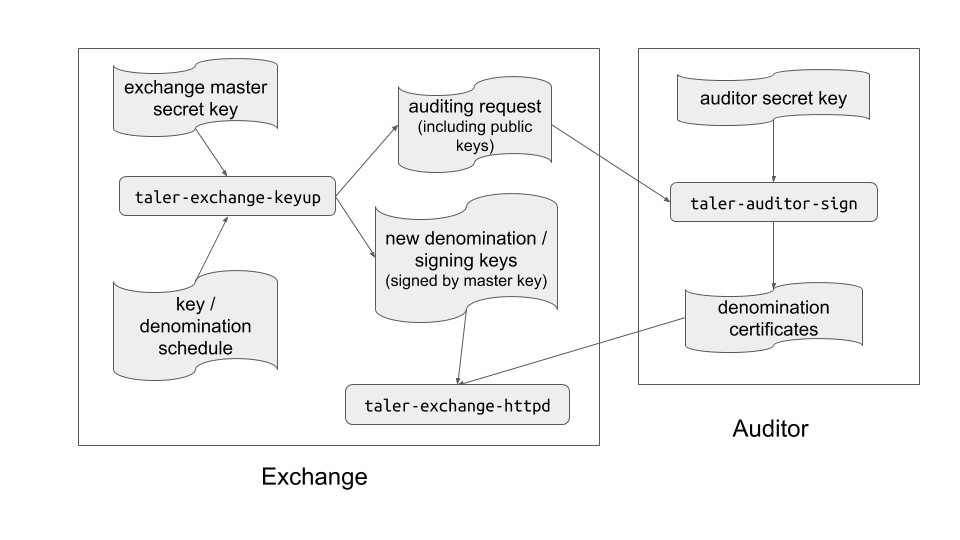
\includegraphics[width=\textwidth]{diagrams/taler-diagram-keyup.png}
    \caption{Data flow for updating the exchange's keys.}
    \label{figure:keyup}
\end{figure}

This process is illustrated in Figure~\ref{figure:keyup}.


\section{Auditor}

The auditor consists of several main components:
\begin{itemize}
 \item the \texttt{taler-auditor-dbinit} tool to setup,
   upgrade or garbage-collect an auditor's database,
 \item the \texttt{taler-auditor-exchange} tool to add an
   exchange to the list of audited exchanges,
 \item the \texttt{taler-auditor-sign} tool to sign an exchange's
   keys to affirm that the auditor is auditing this exchange,
 \item an HTTP service (\texttt{taler-auditor-httpd}) which
   receives deposit confirmations from merchants, and
 \item the \texttt{taler-auditor} script which must be regularly
   run to generate audit reports.
\end{itemize}

\subsection{Database synchronization}

FIXME: describe issue of how to synchronize exchange and auditor
databases, and how we solved it (once we did solve it!) here.

\subsection{The \texttt{taler-auditor} tool}

The \texttt{taler-auditor} script uses several helper processes.  These helper
processes access the exchange's database, either directly (for
exchange-internal auditing as part if its operational security) or over a
replica (in the case of external auditors).

The \texttt{taler-auditor} script ultimately generates a report with the
following information:
\begin{itemize}
  \item Do the operations stored in a reserve's history match the reserve's balance?
  \item Did the exchange record outgoing transactions to the right merchant for
    deposits after the deadline for the payment was reached?
  \item Do operations recorded on coins (deposit, refresh, refund) match the remaining
    value on the coin?
  \item Do operations respect the expiration of denominations?
  \item For a denomination, is the number of pairwise different coin public
    keys recorded in deposit/refresh operations smaller or equal to the number
    of blind signatures recorded in withdraw/refresh operations?
    If this invariant is violated, the corresponding denomination must be revoked.
    %\item Are signatures made by the exchange correct? (no, apparently we don't store signatures)
  \item What is the income if the exchange from different fees?
\end{itemize}

\subsubsection{Report generation}

The \texttt{taler-auditor} script invokes its helper processes, each of
which generates a JSON file with the key findings. The master script then
uses Jinja2 templating to fill a LaTeX template with the key findings, and
runs \texttt{pdflatex} to generate the final PDF.

It is also possible to run the helper processes manually, and given that only
one of them requires read-only access to the bank account of the exchange,
this may be useful to improve parallelism or enhance privilege
separation. Thus, \texttt{taler-auditor} is really only a convenience script.

\subsubsection{Incremental processing}

The operation of all auditor helper processes is incremental.  There is a separate
database to checkpoint the auditing progress and to store intermediate results
for the incremental computation.  Most database tables used by the exchange are
append-only:  rows are only added but never removed or changed.  Tables that
are destructively modified by the exchange only store cached computations based
on the append-only tables.  Each append-only table has a monotonically
increasing row ID.  Thus, the auditor's checkpoint simply consists of the set of
row IDs that were last seen.

\subsubsection{The \texttt{taler-helper-auditor-aggregation}}

This tool checks that the exchange properly aggregates
individual deposits into wire transfers
(see Figure~\ref{fig:deposit:states}).  

The list of invariants checked by this tool thus includes:
\begin{itemize}
\item That the fees charged by the exchange are those
  the exchange provided to the auditor earlier, and that the
  fee calculations (deposit fee, refund fee, wire fee)
  are correct.  Refunds are relevant because refunded amounts
  are not included in the aggregate balance.
\item The sanity of fees, as fees may not exceed the contribution
  of a coin (so the deposit fee cannot be larger than the
  deposited value, and the wire fee cannot exceed the
  wired amount).  Similarly, a coin cannot receive refunds
  that exceed the deposited value of the coin, and the
  deposit value must not exceed the coin's denomination value.
\item That the start and end dates for the wire
  fee structure are sane, that is cover the timeframe without
  overlap or gaps.
\item That denomination signatures on the coins are valid
  and match denomination keys known to the auditor.
\item That the target account of the outgoing aggregate wire
  transfer is well-formed and matches the account specified
  in the deposit.
\item That coins that have been claimed in an aggregation have
  a supporting history.
\item That coins which should be aggregated are listed in an
  aggregation list, and that the timestamps match the
  expected dates.
\end{itemize}


\subsubsection{The \texttt{taler-helper-auditor-coins}}

This helper focuses on checking the history of individual coins (as described
in Figure~\ref{fig:coin:states}), ensuring that the coin is not double-spent
(or over-spent) and that refreshes, refunds and recoups are processed
properly.

Additionally, this tool includes checks for denomination key abuse by
verifying that the value and number of coins deposited in any denomination
does not exceed the value and number of coins issued in that denomination.

Finally, the auditor will also complain if the exchange processes
denominations that it did not properly report (with fee structure) to the
auditor.

The list of invariants checked by this tool thus includes:
\begin{itemize}
\item emergency on denominations because the value or number
  of coins deposited exceeds the value or number of coins
  issued; if this happens, the exchange should revoke the
  respective denomination.
\item various arithmetic inconsistencies from exchanges
  not properly calculating balances or fees during the
  various coin operations (withdraw, deposit, melt, refund);
\item signatures being wrong for denomination key revocation,
  coin denomination signature,
  or coin operations (deposit, melt, refund, recoup)
\item denomination keys not being known to the auditor
\item denomination keys being actually revoked if a recoup
  is granted
\item coins being melted but not (yet) recouped
  (this can be harmless and no fault of the exchange, but
  could also be indicative of an exchange failing to process
  certain requests in a timely fashion)
\end{itemize}


\subsubsection{The \texttt{taler-helper-auditor-deposits}}

This tool verifies that the deposit confirmations reported by merchants
directly to the auditor are also included in the database we got from the
exchange.  This is to ensure that the exchange cannot defraud merchants by
simply not reporting deposits to the auditor or an
exchange signing key being compromised (as described in
Section~\label{sec:signkey:compromise}).

\subsubsection{The \texttt{taler-helper-auditor-reserves}}

This figure checks the exchange's processing of the
balance of an individual reserve, as described
in Figure~\ref{fig:reserve:states}.

The list of invariants checked by this tool thus includes:
\begin{itemize}
\item Correctness of the signatures that legitimized
  withdraw and recoup operations.
\item Correct calculation of the reserve balance given
  the history of operations (incoming wire transfers,
  withdraws, recoups and closing operations)
  involving the reserve.
\item That the exchange closed reserves when required,
  and that the exchange wired the funds back to the
  correct (originating) wire account.
\item Knowledge of the auditor of the denomination keys
  involved in withdraw operations and of the
  applicable closing fee.
\item That denomination keys were valid for use in a
  withdraw operation at the reported time of withdrawal.
\item That denomination keys were eligible for recoup
  at the time of a recoup.
\end{itemize}


\subsubsection{The \texttt{taler-helper-auditor-wire}}

This helper process checks that the incoming and outgoing transfers recorded
in the exchange's database match wire transfers of the underlying bank
account.  To access the transaction history (typically recorded by the bank),
the wire auditor helper is special in that it must be provided the necessary
credentials to access the exchange's bank account.  In a production setting,
this will typically require the configuration and operation of a Nexus
instance (of LibEuFin) at the auditor.

The actual logic of the wire auditor is pretty boring: it goes over all bank
transactions that are in the exchange's database, and verifies that they are
present in the records from the bank, and then it goes over all bank
transactions reported by the bank, and again checks that they are also in the
exchange's database. This applies for both incoming and outgoing wire
transfers.  The tool reports any inconsistencies, be they in terms of wire
transfer subject, bank accounts involved, amount that was transferred, or
timestamp.

For incoming wire transfers, this check protects against the following
failures: An exchange reporting the wrong amount may wrongfully allow or
refuse the withdrawal of coins from a reserve. The wrong wire transfer subject
might allow the wrong wallet to withdraw, and reject the rightful owner.  The
wrong bank account could result in the wrong recipient receiving funds if the
reserve is closed. Timestamp differences are usually pretty harmless, and
small differences may even occur due to rounding or clock synchronization
issues. However, they are still reported as they may be indicative of other
problems.

For outgoing wire transfers, the implications arising from an exchange making
the wrong wire transfers should be obvious.

The list of invariants checked by this tool thus includes:
\begin{itemize}
\item The exchange correctly listing all incoming wire transfers.
\item The bank/Nexus having correctly suppressed incoming wire
  transfers with non-unique wire transfer subjects, and having
  assigned each wire transfer a unique row ID/offset.
\item The exchange correctly listing all outgoing wire transfers
  including having the appropriate justifications (aggregation
  or reserve closure) for the respective amounts and target accounts.
\item Wire transfers that the exchange has failed to execute that
  were due. Note that small delays here can be normal as
  wire transfers may be in flight.
\end{itemize}


\subsection{The Auditor's HTTP service}

The auditor exposes a web server with the \texttt{taler-auditor-httpd}
process.  Currently, it shows a website that allows the customer to add the
auditor to the list of trusted auditors in their wallet.

It also exposes an endpoint for merchants to submit deposit confirmations.
These merchant-submitted deposit confirmations are checked against the deposit
permissions in the exchange's database to detect compromised signing keys or
missing writes, as described in
Section~\ref{sec:compromised-signing-key-detection}.

In the future, we plan for the auditor to expose additional endpoints where
wallets and merchant backends can submit (cryptographic) proofs of
missbehavior from an exchange. The goal would be to automatically verify the
proofs, take corrective action by including the information in the audit
report and possibly even compensating the victim.


\section{Merchant Backend}

\begin{figure}
    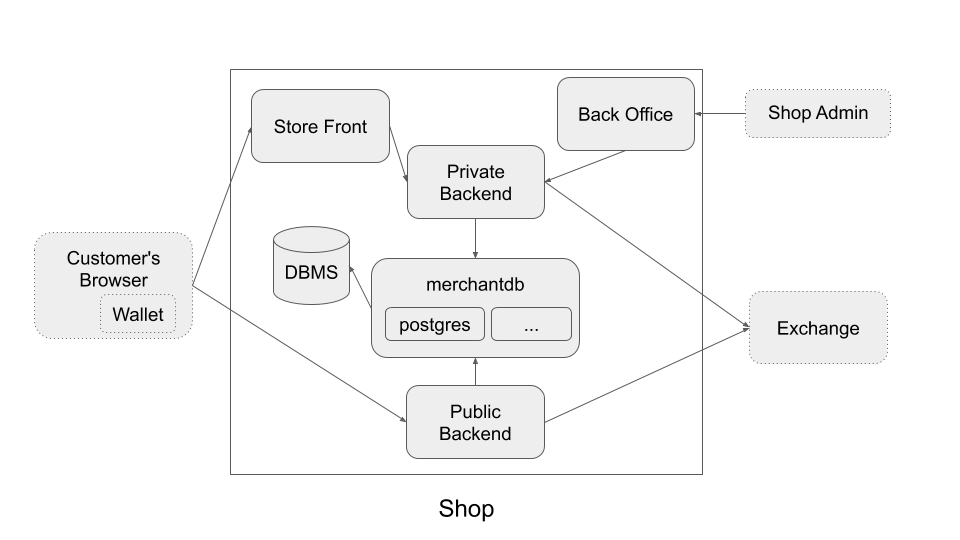
\includegraphics[width=\textwidth]{diagrams/taler-diagram-merchant.png}
    \caption{Architecture of the merchant reference implementation}
\end{figure}

The Taler merchant backend is a component that abstracts away the details of
processing Taler payments and provides a simple HTTP API.  The merchant backend
handles cryptographic operations (signature verification, signing), secret
management and communication with the exchange.

The backend API\footnote{See \url{https://docs.taler.net/api/} for the full documentation}
is divided into two types of HTTP endpoints:
\begin{enumerate}
  \item Functionality that is accessed internally by the merchant.  These APIs typically
    require authentication and/or are only accessible from within the private
    network of the merchant.
  \item Functionality that is exposed publicly on the Internet and accessed by the customer's wallet and browser.
    % FIXME: talk about proxying
\end{enumerate}

A typical merchant has a \emph{storefront} component that customers visit with
their browser, as well as a \emph{back office} component that allows the
merchant to view information about payments that customers made and that integrates
with other components such as order processing and shipping.

\subsection{Processing payments}\label{sec:processing-payments}

To process a payment, the storefront first instructs the backend to create an
\emph{order}.  The order contains information relevant to the purchase, and is
in fact a subset of the information contained in the contract terms.  The
backend automatically adds missing information to the order details provided by
the storefront.  The full contract terms can only be signed once the customer
provides the claim public key for the contract.

Each order is uniquely identified by an order ID, which can be chosen by the
storefront or automatically generated by the backend.

The order ID can be used to query the status of the payment.  If the customer
did not pay for an order ID yet, the response from the backend includes a
payment redirect URL.  The storefront can redirect the customer to this
payment redirect URL; visiting the URL will trigger the customer's
browser/wallet to prompt for a payment.

To simplify the implementation of the storefront, the merchant backend can
serve a page to the customer's browser that triggers the payment via the HTTP
402 status code and the corresponding headers, and provides a fallback (in the
form of a \texttt{taler:pay} link) for loosely integrated browsers.
When checking the status of a payment that is not settled yet, the response from the merchant backend
will contains a payment redirect URL.  The storefront redirects the browser to this URL,
which is served by the merchant backend and triggers the payment.

The code snippet shown in Figure~\ref{fig:merchant-donations-code} implements
the core functionality of a merchant frontend that prompts the customer for a
donation (upon visiting \texttt{/donate} with the right query parameters) and
shows a donation receipt on the fulfillment page with URL \texttt{/receipt}.
The code snippet is written in Python and uses the Flask library\footnote{\url{http://flask.pocoo.org/}} to process HTTP requests.
The helper functions \texttt{backend\_post}
and \texttt{backend\_get} make an HTTP \texttt{POST}/\texttt{GET} request to the merchant backend, respectively,
with the given request body / query parameters.

\begin{figure}
\lstinputlisting[language=Python,basicstyle=\footnotesize]{snippets/donations.py}
\caption[Code snippet for merchant frontend]{Code snippet with core functionality of a merchant frontend to accept donations.}
\label{fig:merchant-donations-code}
\end{figure}


\subsection{Back Office APIs}

The back office API allows the merchant to query information about the history
and status of payments, as well as correlate wire transfers to the merchant's
bank account with the respective GNU Taler payment.  This API is necessary to
allow integration with other parts of the merchant's e-commerce infrastructure.

%\subsection{Instances}
%Merchant instances allow one deployment of the merchant backend to host more
%than one logical merchant.  

\subsection{Example Merchant Frontends}

We implemented the following applications using the merchant backend API.

\begin{description}
  \item[Blog Merchant] The blog merchant's landing page has a list of article titles with a teaser.
    When following the link to the article, the customer is asked to pay to view the article.
  \item[Donations]  The donations frontend allows the customer to select a project to donate to.
    The fulfillment page shows a donation receipt.
  \item[Codeless Payments]  The codeless payment frontend is a prototype for a
    user interface that allows merchants to sell products on their website
    without having to write code to integrate with the merchant backend.
    Instead, the merchant uses a web interface to manage products and their
    available stock.  The codeless payment frontend then creates an HTML snippet with a payment
    button that the merchant can copy-and-paste integrate into their storefront.
  \item[Survey]  The survey frontend showcases the tipping functionality of GNU Taler.
    The user fills out a survey and receives a tip for completing it.
  \item[Back office] The example back-office application shows the history and
    status of payments processed by the merchant.
\end{description}

The code for these examples is available at \url{https://git.taler.net/} in the
repositories \texttt{blog}, \texttt{donations}, \texttt{codeless}, \texttt{survey}
and \texttt{backoffice} respectively.


\section{Wallet}

\begin{figure}
    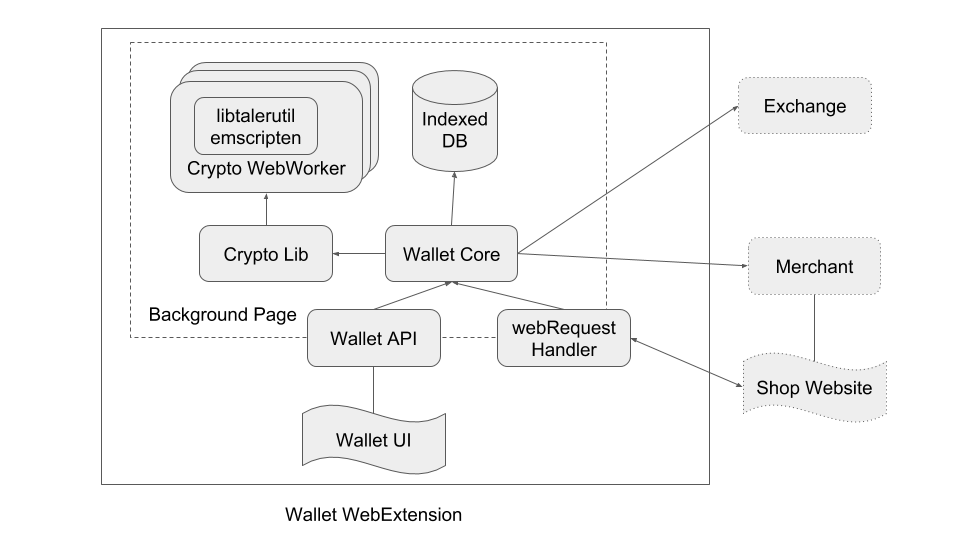
\includegraphics[width=\textwidth]{diagrams/taler-diagram-wallet.png}
    \caption{Architecture of the wallet reference implementation}
\end{figure}

The wallet manages the customer's reserves and coins, lets the customer view
and pay for contracts from merchants.  It can be seen in operation in
Section~\ref{sec:intro:ux}.

The reference implementation of the GNU Taler wallet is written in the
TypeScript language against the WebExtension API%
\footnote{\url{https://developer.mozilla.org/en-US/docs/Mozilla/Add-ons/WebExtensions}}, a cross-browser mechanism for
browser extensions.  The reference wallet is a ``tightly integrated'' wallet, as it directly hooks into
the browser to process responses with the HTTP status code ``402 Payment Required''.

Many cryptographic operations needed to implement the wallet are not commonly
available in a browser environment.  We cross-compile the GNU Taler utility
library written in C as well as its dependencies (such as libgcrypt) to asm.js
(and WebAssembly on supported platforms) using the LLVM-based emscripten
toolchain \cite{zakai2011emscripten}.

Cryptographic operations run in an isolated process implemented as a
WebWorker.\footnote{\url{https://html.spec.whatwg.org/}}  This design allows
the relatively slow cryptographic operations to run concurrently in the
background in multiple threads.  Since the crypto WebWorkers are started on-demand,
the wallet only uses minimal resources when not actively used.

\subsection{Optimizations}\label{sec:wallet-optimizations}
To improve the perceived performance of cryptographic operations,
the wallet optimistically creates signatures in the background
while the user is looking at the ``confirm payment'' dialog.  If the user does
not accept the contract, these signatures are thrown away instead of being sent
to the merchant.  This effectively hides the latency of the
most expensive cryptographic operations, as they are done while the user
consciously needs to make a decision on whether to proceed with a payment.


\subsection{Coin Selection}
The wallet hides the implementation details of fractionally spending different
denomination from the user, and automatically selects which denominations to
use for withdrawing a given amount, as well as which existing coins to
(partially) spend for a payment.

Denominations for withdrawal are greedily selected, starting with the largest
denomination that fits into the remaining amount to withdraw.  Coin selection
for spending proceeds similarly, but first checks if there is a single coin
that can be partially spent to cover the whole amount.  After each payment, the
wallet automatically refreshes coins with a remaining amount large enough to be
refreshed.  We discuss a simple simulation of the current coin selection algorithm
in Section~\ref{sec:coins-per-transaction}.

A more advanced coin selection would also consider the fee structure of the
exchange, minimizing the number of coins as well as the fees incurred by the
various operations.  The wallet could additionally learn typical amounts that
the user spends, and adjust withdrawn denominations accordingly to further
minimize costs.  An opposing concern to the financial cost is the anonymity of
customers, which is improved when the spending behavior of wallets is as
similar as possible.

% FIXME: what about anonymity effects of coin selection?

\subsection{Wallet Detection}
When websites such as merchants or banks try to signal the Taler wallet---for example,
to request a payment or trigger reserve creation---it is possible that the
customer simply has no Taler wallet installed.  To accommodate for this situation in a
user-friendly way, the HTTP response containing signaling to wallet should
contain as response body an HTML page with (1) a \texttt{taler:} link to
manually open loosely integrated wallets and (2) instructions on how to install
a Taler wallet if the user does not already have one.

It might seem useful to dynamically update page content depending on whether
the Taler wallet is installed, for example, to hide or show a ``Pay with Taler''
or ``Withdraw to Taler wallet'' option.  This functionality cannot be provided
in general, as only the definitive presence of a wallet can be detected, but
not its absence when the wallet is only loosely integrated in the user's
browser via a handler for the \texttt{taler:} URI scheme.

We nevertheless consider the ability to know whether a customer has definitely
installed a Taler wallet useful (if only for the user to confirm that the
installation was successful), and expose two APIs to query this.  The first one
is JavaScript-based and allows to register a callback for the when
presence/absence of the wallet is detected.  The second method works without
any JavaScript on the merchant's page, and uses CSS~\cite{sheets1998level} to dynamically show/hide
element on the page marked with the special \texttt{taler-installed-show} and
\texttt{taler-installed-hide} CSS classes, whose visibility is changed when
a wallet browser extension is loaded.

Browser fingerprinting \cite{mulazzani2013fast} is a concern with any
additional APIs made available to websites, either by the browser itself or by
browser extensions.  Since a website can simply try to trigger a payment to
determine whether a tightly integrated Taler wallet is installed, one bit of
additional fingerprinting information is already available through the usage of
Taler.  The dynamic detection methods do not, however, expose any information
that is not already available to websites by signaling the wallet through HTTP
headers.

\subsection{Backup and Synchronization}
While users can manually import and export the state of the wallet, at the time
of writing this, automatic backup and synchronization between wallets is not
implemented yet.  We discuss the challenges with implementing backup and
synchronization in a privacy-preserving manner in
Chapter~\ref{sec:future-work-backup-sync}.


\subsection{Wallet Liquidation}
If a customer wishes to stop using GNU Taler, they can deposit the remaining
coins in their wallet back to their own bank account.  We call this process
\emph{liquidation}.

In deployments with relatively lenient KYC regulation, the normal deposit
functionality used by merchants is used for wallet liquidation.  The wallet
simply acts as a merchant for one transaction, and asks the exchange to deposit
the coins into the customer's bank account.

However in deployments with strict KYC regulations, the customer would first
have to register and complete a KYC registration procedure with the exchange.
To avoid this, liquidation can be implemented as a modified deposit, which
restricts the payment to the bank account that was used to create a reserve of
the customer.

The exchange cannot verify that a coin that is being liquidated actually
originated the reserve that the customer claims it originated from, unless the
user reveals the protocol transcripts for withdrawal and refresh operations on
that coin, violating their privacy.  Instead, each reserve tracks the amount
that was liquidated into it, and the exchange rejects a liquidation request if
the liquidated amount exceeds the amount that was put into the reserve.  Note
that liquidation does not refill the funds of a reserve, but instead triggers a
bank transfer of the liquidated amount to the bank account that
created the reserve.


\subsection{Wallet Signaling}
We now define more precisely the algorithm that the wallet executes when a
website signals to that wallet that an operation related to payments should be
triggered, either by opening a \texttt{taler:pay} URL or by responding
with HTTP 402 and at least one Taler-specific header.

% FIXME:  need to specify what happens when gateway_origin="", for example when triggered
% via URL
The steps to process a payment trigger are as follows.  The algorithm takes the
following parameters: \texttt{current\_url} (the URL of the page that
raises the 402 status or \texttt{null} if triggered by a \texttt{taler:pay} URL),
\texttt{contract\_url}, \texttt{resource\_url}, \texttt{session\_id},
\texttt{offer\_url}, \texttt{refund\_url}, \texttt{tip\_token} (from the
``Taler-\dots'' headers or \emph{taler:pay} URL parameters respectively)
\begin{enumerate}
  \item If \texttt{resource\_url} a non-empty string, set \texttt{target\_url} to \texttt{resource\_url},
    otherwise set \texttt{target\_url} to \texttt{current\_url}.
  \item If \texttt{target\_url} is empty, stop.
  \item If there is an existing payment $p$ whose
    fulfillment URL equals \texttt{target\_url} and either \texttt{current\_url} is \texttt{null}
    or \texttt{current\_url} has the same origin as
    either the fulfillment URL or payment URL in the contract terms, then:
    \begin{enumerate}[label*=\arabic*.]
      \item If \texttt{session\_id} is non-empty and the last session ID for payment $p$ was recorded
        in the wallet with session signature $sig$, construct a fulfillment instance URL from $sig$ 
        and the order ID of $p$.
      \item Otherwise, construct an extended fulfillment URL from the order ID of $p$.
      \item Navigate to the extended fulfillment URL constructed in the previous step and stop.
    \end{enumerate}
  \item If \texttt{contract\_url} is a non-empty URL, execute the steps for
    processing a contract URL (with \texttt{session\_id}) and stop.
  \item If \texttt{offer\_url} is a non-empty URL, navigate to it and stop.
  \item If \texttt{refund\_url} is a non-empty URL, process the refund and stop.
  \item If \texttt{tip\_url} is a non-empty URL, process the tip and stop.
\end{enumerate}

For interactive web applications that request payments, such as games or single
page apps (SPAs), the payments initiated by navigating to a page with HTTP
status code 402 are not appropriate, since the state of the web application is
destroyed by the navigation.  Instead the wallet can offer a JavaScript-based
API, exposed as a single function with a subset of the parameters of the
402-based payment: \texttt{contract\_url}, \texttt{resource\_url},
\texttt{session\_id} \texttt{refund\_url}, \texttt{offer\_url},
\texttt{tip\_token}.  Instead of navigating away, the result of the operation
is returned as a JavaScript promise (either a payment receipt, refund
confirmation, tip success status or error).  If user input is required (e.g., to
ask for a confirmation for a payment), the page's status must not be destroyed.
Instead, an overlay or separate tab/window displays the prompt to the user.
% FIXME:  should be specify the full algorithm for JS payments?

% FIXME talk about clickjacking



\newcommand\inecc{\in \mathbb{Z}_{|\mathbb{E}|}}
\newcommand\inept{\in {\mathbb{E}}}
\newcommand\inrsa{\in \mathbb{Z}_{|\mathrm{dom}(\FDH_K)|}}

\section{Cryptographic Protocols}

\def\HKDF{\textrm{HKDF}}
\def\KDF{\textrm{KDF}}
\def\FDH{\textrm{FDH}}
\newcommand{\iseq}{\stackrel{?}{=}}
\newcommand{\iseqv}{\stackrel{?}{\equiv}}
\newcommand{\pccheck}{\mathbf{check}\ }

In this section, we describe the main cryptographic protocols for Taler in more
detail.  The more abstract, high-level protocols from
Section~\ref{sec:crypto:instantiation} are instantiated and and embedded in
concrete protocol diagrams that can hopefully serve as a reference for
implementors.

For ease of presentation, we do not provide a bit-level description of the
cryptographic protocol.  Some details from the implementation are left out,
such as fees, additional timestamps in messages and checks for the expiration
of denominations. Furthermore, we do not specify the exact responses in the
error cases, which in the actual implementation should include signatures that
could be used during a legal dispute.  Similarly, the actual implementation
contains some additional signatures on messages sent that allow to prove to a
third party that a participant did not follow the protocol.

As we are dealing with financial transactions, we explicitly describe whenever
entities need to safely write data to persistent storage.  As long as the data
persists, the protocol can be safely resumed at any step.  Persisting data is
cumulative, that is an additional persist operation does not erase the
previously stored information.

The implementation also records additional entries in the exchange's database
that are needed for auditing.

\subsection{Preliminaries}
In our protocol definitions, we write $\mathbf{check}\ \mathrm{COND}$ to abort
the protocol with an error if the condition $\mathrm{COND}$ is false.

We use the following algorithms:
\begin{itemize}
\item $\algo{Ed25519.Keygen}() \mapsto \langle \V{sk}, \V{pk} \rangle$
    to generate an Ed25519 key pair.
 \item $\algo{Ed25519.GetPub}(\V{sk}) \mapsto \V{pk}$ to derive the public key from
    an Ed25519 public key.
 \item $\algo{Ed25519.Sign}(\V{sk}, m) \mapsto \sigma$ to create a signature $\sigma$
    on message $m$ using secret key $\V{sk}$.
 \item $\algo{Ed25519.Verify}(\V{pk}, \sigma, m) \mapsto b$ to check if $\sigma$ is
   a valid signature from $\V{pk}$ on message $m$.
 \item $\mathrm{HKDF}(n, k, s) \mapsto m$ is the HMAC-based key derivation function \cite{rfc5869},
   producing an output $m$ of $n$ bits from the input key material $k$ and salt $s$.
\end{itemize}

We write $\mathbb{Z}^*_N$ for the multiplicative group of integers modulo $N$.
Given an $r \in \mathbb{Z}^*_N$, we write $r^{-1}$ for the multiplicative
inverse modulo $N$ of $r$.

We write $H(m)$ for the SHA-512 hash of a bit string,
and $\FDH(N,m)$ for the full domain hash that maps the bit string $m$ to an element
of $\mathbb{Z}^*_N$.

The expression $x \randsel X$ denotes uniform random selection of an element
$x$ from set $X$.  We use $\algo{SelectSeeded}(s, X) \mapsto x$ for pseudo-random uniform
selection of an element $x$ from set $X$ and seed $s$.  Here, the result is deterministic for fixed inputs $s$ and $X$.

The exchange's denomination signing key pairs $\{\langle \V{skD}_i, \V{pkD}_i \rangle \}$ are RSA keys pairs,
and thus $\V{pkD}_i = \langle e_i, N_i \rangle$, $\V{skD_i} = d_i$.  We write $D(\V{pkD}_i)$ for the
financial value of the denomination $\V{pkD}_i$.

% FIXME: explain RSA keys of exchange


\subsection{Withdrawing}
The withdrawal protocol is defined in Figure~\ref{fig:withdraw-protocol}.
The following additional algorithms are used, which we only define informally here:
\begin{itemize}
  \item $\algo{CreateBalance}(W_p, v) \mapsto \bot$ is used by the exchange,
    and has the side-effect of creating a reserve record with balance $v$
    and reserve public key (effectively the identifier of the reserve) $W_p$.
  \item $\algo{GetWithdrawR}(\rho) \mapsto \{\bot,\overline{\sigma}_C\}$
    is used by the exchange, and checks
    if there is an existing withdraw request $\rho$.  If the existing request
    exists, the existing blind signature $\overline{\sigma}_C$ over
    coin $C$ is returned.  On a fresh request, $\bot$ is
    returned.
  \item $\algo{BalanceSufficient}(W_s,\V{pkD}_t) \mapsto b$ is used by the exchange, and
    returns true if the balance in the reserve identified by $W_s$ is sufficient to
    withdraw at least one coin if denomination $\V{pkD}_t$.
  \item $\algo{DecreaseBalance}(W_s,\V{pkD}_t) \mapsto \bot$ is used by the exchange, and
    decreases the amount left in the reserve identified by $W_s$ by the amount $D(\V{pkD}_t)$
    that the denomination $\V{pkD}_t$ represents.
\end{itemize}

\begin{figure}
\centering
\fbox{%
\pseudocode[codesize=\small]{%
\textbf{Customer} \< \< \textbf{Exchange} \\
  \text{Knows } \{ \langle e_i,N_i \rangle \} = \{\V{pkD}_i\} \< \< \text{Knows } \{ \langle \V{skD}_i, \V{pkD}_i \rangle \} \pclb
\pcintertext[dotted]{Create Reserve} 
\langle w_s, W_p \rangle \leftarrow \algo{Ed25519.Keygen}() \< \< \\
\text{Persist reserve } \langle w_s,v \rangle \< \< \\
  \< \sendmessageright{top={Bank transfer}, bottom={(subject: $W_p$, amount: $v$)},style=dashed} \< \\
  \< \< \algo{CreateBalance}(W_p, v) \pclb
\pcintertext[dotted]{Prepare Withdraw}
\text{Choose $t$ with $\V{pkD}_t \in \{\V{pkD}_i\}$} \< \< \\
\langle c_s, C_p \rangle \leftarrow \algo{Ed25519.Keygen}() \< \< \\
  r \randsel \mathbb{Z}^*_N \< \< \\
  \text{Persist planchet } \langle c_s, r \rangle \< \< \pclb
\pcintertext[dotted]{Execute Withdraw}
\overline{m} := \FDH(N_t, C_p) \cdot r^{e_t} \bmod N_t \< \< \\
\rho_W := \langle \V{pkD}_t, \overline{m} \rangle \< \< \\
\sigma_W := \algo{Ed25519.Sign}(w_s, \rho_W) \< \< \\
\< \sendmessageright*{\rho := \langle W_p, \sigma_W, \rho_W \rangle} \< \\
  \< \< \pccheck \V{pkD}_t \in  \{ \V{pkD}_i \} \\
\< \< \pccheck \algo{Ed25519.Verify}(W_p,\rho_W,\sigma_W) \\
\< \< x \leftarrow \algo{GetWithdraw}(\rho) \\
\< \< \pcif x \iseq \bot \\
\< \< \t \pccheck \algo{BalanceSufficient}(W_p,\V{pkD}_t) \\
\< \< \t \algo{DecreaseBalance}(W_p, \V{pkD}_t) \\
\< \< \t \text{Persist withdrawal $\rho$} \\
\< \< \t \overline{\sigma}_C := (\overline{m})^{\V{skD}_t} \bmod N_t \\
\< \< \pcelse \\
\< \< \t \overline{\sigma}_C := x \\
\< \sendmessageleft*{\overline{\sigma}_C} \< \\
\sigma_C := r^{-1}\overline{\sigma}_C \< \< \\
\pccheck \sigma_C^{e_t} \iseqv_{N_t} \FDH(N_t, C_p) \< \< \\
\text{Persist coin $\langle \V{pkD}_t, c_s, C_p, \sigma_C \rangle$}  \< \< \\
}
}
\caption[Withdraw protocol diagram.]{Withdrawal protocol diagram.}
\label{fig:withdraw-protocol}
\end{figure}

\subsection{Payment transactions}
The payment protocol is defined in two parts.  First, the spend protocol in
Figure~\ref{fig:payment-spend} defines the interaction between a merchant and
a customer.  The customer obtains the contract terms (as $\rho_P$) from the
merchant, and sends the merchant deposit permissions as a payment.  The deposit protocol
in Figure~\ref{fig:payment-deposit} defines how subsequently the merchant sends the
deposit permissions to the exchange to detect double-spending and ultimately
to receive a bank transfer from the exchange.

Note that in practice the customer can also execute the deposit
protocol on behalf of the merchant. This is useful in situations where
the customer has network connectivity but the merchant does not. It
also allows the customer to complete a payment before the payment
deadline if a merchant unexpectedly becomes unresponsive, allowing the
customer to later prove that they paid on time.

We limit the description to one exchange here, but in practice, the merchant
communicates to the customer the exchanges that it supports, in addition to the
account information $A_M$ that might differ between exchanges.

We use the following algorithms, defined informally here:
\begin{itemize}
 \item $\algo{SelectPayCoins}(v, E_M) \mapsto \{ \langle \V{coin}_i, f_i \rangle \}$ selects
   fresh coins (signed with denomination keys from exchange $E_M$)
   to pay for the amount $v$.  The result is a set of coins
   together with the fraction of each coin that must be spent such that
   the amounts contributed by all coins sum up to $v$.
 \item $\algo{MarkDirty}(\V{coin}, f) \mapsto \bot$ subtracts the fraction $f$ from the
   available amount left on a coin, and marks the coin as dirty (to trigger refreshing
   in case $f$ is below the denomination value).  Thus, assuming the coin has
   any residual value, the customer's wallet will do a refresh on $\V{coin}$
   and not use it for further payments.  This provides unlinkability of transactions
   made with change arising from paying with fractions of a coin's denomination.
 \item $\algo{Deposit}(E_M, D_i) \mapsto b$ executes the second part of the payment protocol
   (i.e., the deposit) with exchange $E_M$, using deposit permission $D_i$.
 \item $\algo{GetDeposit}(C_p, h) \mapsto \{\bot,\rho_{(D,i)}\}$ checks in the exchange's database
    for an existing processed deposit permission on coin $C_p$ for the contract
    identified by $h$.  The algorithm returns the existing deposit permission $\rho_{(D,i)}$, or $\bot$ if a
    matching deposit permission is not recorded.
 \item $\algo{IsOverspending}(C_p, \V{pkD}, f) \mapsto b$ checks in the exchange's database
   if there if at least the fraction $f$ of the coin $C_p$ of denomination $\V{pkD}$ is still available
   for use, based on existing spend/withdraw records of the exchange.
 \item $\algo{MarkFractionalSpend}(C_p, f) \mapsto \bot$ adds a spending
   record to the exchanges database, indicating
   that fraction $f$ of coin $C_p$ has been spent (in addition to
   existing spending/refreshing records).
 \item $\algo{ScheduleBankTransfer}(A_M, f, \V{pkD}, h_c) \mapsto \bot$
   schedules a bank transfer from the exchange to
   the account identified by $A_M$, for subject $h_c$ and for the amount $f\cdot D(\V{pkD})$.
   % NOTE: actual implementation avoids multiplication (messy!) and would
   % simply require f \le D(\V{pkD})!
\end{itemize}


\begin{figure}
\centering
\fbox{%
\pseudocode[codesize=\footnotesize]{%
\textbf{Customer} \< \< \textbf{Merchant} \\
\text{Knows } \V{pkM} \< \< \text{Knows } \langle \V{pkM}, \V{skM} \rangle \\
\< \sendmessageright{top={Select product/service},style=dashed} \< \\
\< \< \text{Determine:} \\
\< \< \text{$\bullet$ } v \text{ (price) } \\
\< \< \text{$\bullet$ } E_M \text{ (exchange) } \\
\< \< \text{$\bullet$ } A_M \text{ (acct.) } \\
\< \< \text{$\bullet$ } \V{info} \text{ (free-form details) } \\
\< \sendmessageleft{top={Request payment},style=dashed} \< \\
\langle p_s, P_p \rangle \leftarrow \algo{Ed25519.Keygen}() \< \< \\
\text{Persist ownership identifier } p_s \< \< \\
\< \sendmessageright*{P_p} \< \\
  \< \< \rho_P := \langle E_M, A_M, \V{pkM}, H(\langle v, \V{info}\rangle), P_p \rangle \\
\< \< \sigma_P := \V{Ed25519.Sign}(\V{skM}, \rho_P) \\
\< \sendmessageleft*{\rho_P, \sigma_P, v, \V{info}} \< \\
  \langle M, A_M, \V{pkM}, h', P_p' \rangle := \rho_P \< \< \\
\pccheck \algo{Ed25519.Verify}(pkM, \sigma_P, \rho_P) \< \< \\
\pccheck P_p' \iseq P_p \< \< \\
\pccheck h' \iseq H(\langle v, \V{info} \rangle ) \< \< \\
\V{cf} \leftarrow \algo{SelectPayCoins}(v, E_M) \< \< \\
\pcfor \langle \V{coin_i,f_i} \rangle \in \V{cf} \< \< \\
\t \algo{MarkDirty}(\V{coin}_i, f_i) \< \< \\
\t \langle c_s, C_p, \V{pkD}, \sigma_C \rangle := \V{coin}_i \< \< \\
  \t \rho_{(D,i)} := \langle C_p, \V{pkD}, \sigma_C, f_i, H(\rho_P), A_M, \V{pkM} \rangle \< \< \\
\t \sigma_{(D,i)} := \V{Ed25519.Sign}(c_s, \rho_{(D,i)}) \< \< \\
  \text{Persist } \langle \sigma_P, \V{cf}, \rho_P, \rho_{(D,i)}, \sigma_{(D,i)}, v, \V{info} \rangle \< \<\\
\< \sendmessageright*{ \mathcal{D} := \{\langle \rho_{(D,i)}, \sigma_{(D,i)}\rangle \}} \< \\
\< \< \pcfor D_i \in \mathcal{D} \\
\< \< \t \pccheck \algo{Deposit}(E_M, D_i) \\
}
}
\caption[Spend protocol diagram.]{Spend Protocol executed between customer and merchant for the purchase
  of an article of price $v$ using coins from exchange $E_M$. The merchant has
  provided his account details to the exchange under an identifier $A_M$.
  The customer can identify themselves as the one who received the offer
  using $p_s$.
  %This prevents multiple customers from legitimately paying for the
  %same article and potentially exhausting stocks.
}
\label{fig:payment-spend}
\end{figure}

\begin{figure}
\centering
\fbox{%
\pseudocode[codesize=\small]{%
\textbf{Customer/Merchant} \< \< \textbf{Exchange} \\
\text{Knows } \V{pkESig} \< \< \text{Knows } \V{skESig}, \V{pkESig}, \{ \V{pkD}_i \} \\
\text{Knows } D_i = \langle \rho_{(D,i)}, \sigma_{(D,i)} \rangle \< \< \\
\< \sendmessageright*{ D_i } \< \\
\< \< \langle \rho_{(D,i)}, \sigma_{(D,i)} \rangle := D_i \\
  \< \< \langle C_p, \V{pkD}, \sigma_C, f_i, h, A_M, \V{pkM} \rangle := \rho_{(D,i)} \\
\< \< \pccheck \V{pkD} \in \{ \V{pkD}_i \} \\
\< \< \langle e, N \rangle := \V{pkD} \\
\< \< \pccheck \algo{Ed25519.Verify}(C_p, \sigma_{(D,i)}, \rho_{(D,i)}) \\
\< \< x \leftarrow \algo{GetDeposit}(C_p, h) \\
\< \< \pcif x \iseq \bot  \\
\< \< \t \pccheck \sigma_C^{e} \iseqv_N \FDH(N, C_p) \\
\< \< \t \pccheck \neg\algo{IsOverspending}(C_p, \V{pkD}, f) \\
\< \< \t \text{Persist deposit-record } D_i \\
\< \< \t \algo{MarkFractionalSpend}(C_p, f) \\
\< \< \t \algo{ScheduleBankTransfer}(A_M, f, \V{pkD}, h_c) \\
\< \< \pcelse \\
\< \< \t \pccheck x \iseq \rho_{(D,i)} \\
\< \< \sigma_{DC} \leftarrow \algo{Ed25519.Sign}(\V{pkESig}, \rho_{(D,i)}) \\
\< \sendmessageleft*{ \sigma_{DC} } \< \\
\pccheck \algo{Ed25519.Verify} \\{}\qquad(\V{pkESig}, \sigma_{DC}, \rho_{(D,i)}) \< \< \\
}
}
\caption[Deposit protocol diagram.]{Deposit Protocol run for each deposited coin $D_i \in {\cal D}$ with the
  exchange that signed the coin.}
\label{fig:payment-deposit}
\end{figure}


\subsection{Refreshing and Linking}
The refresh protocol is defined in Figures~\ref{fig:refresh-part1} and
\ref{fig:refresh-part2}.  The refresh protocol allows the customer to
obtain change for the remaining fraction of the value of a coin.  The
change is generated as a fresh coin that is unlinkable to the dirty
coin to anyone except for the owner of the dirty coin.

A na\"ive implementation of a refresh protocol that just gives the customer a
new coin could be used for peer-to-peer transactions that hides income from tax
authorities.  Thus, (with probability $(1-1/\kappa)$) the refresh protocol
records information that allows the owner of the original coin to obtain the
refreshed coin from the original coin via the linking protocol (illustrated in
Figure~\ref{fig:link}).

We use the following algorithms, defined informally here:
\begin{itemize}
  \item \algo{RefreshDerive} is defined in Figure~\ref{fig:refresh-derive}.
  \item $\algo{GetOldRefresh}(\rho_{RC}) \mapsto \{\bot,\gamma\}$ returns the past
    choice of $\gamma$ if $\rho_{RC}$ is a refresh commit message that has been seen before,
    and $\bot$ otherwise.
  \item $\algo{IsConsistentChallenge}(\rho_{RC}, \gamma) \mapsto \{ \bot,\top \}$ returns
    $\top$ if no refresh-challenge has been persisted for the refresh operation by commitment
    $\rho_{RC}$ or $\gamma$ is consistent with the persisted (and thus previously received) challenge;
    returns $\bot$ otherwise.
  \item $\algo{LookupLink}(C_p) \mapsto \{ \langle \rho_{L}^{(i)}, \sigma_L^{(i)},
  \overline{\sigma}_C^{(i)} \rangle \}$ looks up refresh records on coin with public key $C_p$ in
    the exchange's database and returns the linking message $\rho_L^{(i)}$, linking
    signature $\sigma_L^{(i)}$ and blinded signature $\overline{\sigma}_C^{(i)}$ for each refresh
    record $i$.
\end{itemize}


\begin{figure}
\centering
\fbox{%
\procedure[codesize=\small]{$\algo{RefreshDerive}(s, \langle e, N \rangle, C_p)$}{%
t := \HKDF(256, s, \texttt{"t"}) \\
T := \algo{Curve25519.GetPub}(t) \\
x := \textrm{ECDH-EC}(t, C_p)  \\
r := \algo{SelectSeeded}(x, \mathbb{Z}^*_{N})  \\
c_s := \HKDF(256, x, \texttt{"c"}) \\
C_p := \algo{Ed25519.GetPub}(c_s)  \\
\overline{m} := r^{e}\cdot C_p \mod N \\
\pcreturn \langle t, T, x, c_s, C_p, \overline{m} \rangle
}
}
\caption[RefreshDerive algorithm]{The RefreshDerive algorithm running with the seed $s$ on dirty coin $C_p$ to
   generate a fresh coin to be later signed with denomination key $pkD := \langle e,N\rangle$.}
\label{fig:refresh-derive}
\end{figure}


\begin{figure}
\centerline{
\fbox{%
\pseudocode[codesize=\footnotesize]{%
\textbf{Customer} \< \< \textbf{Exchange} \\
\text{Knows } \{ \V{pkD}_i \} \< \< \text{Knows } \{\langle  \V{skD}_i, \V{pkD}_i \rangle \}  \\
\text{Knows } \V{coin}_0 = \langle \V{pkD}_0, c_s^{(0)}, C_p^{(0)}, \sigma_{C}^{(0)} \rangle \< \<  \\
\text{Select } \langle N_t, e_t \rangle := \V{pkD}_t \in \{ \V{pkD}_i \} \< \<  \\
\pcfor i = 1,\dots,\kappa \< \<  \\
\t s_i \randsel \{0,1\}^{256} \< \<  \\
\t X_i := \algo{RefreshDerive}(s_i, \V{pkD}_t, C_p^{(0)}) \< \< \\
\t (t_i, T_i, x_i, c_s^{(i)}, C_p^{(i)}, \overline{m}_i) := X_i \< \< \\
h_T := H(T_1,\dots,T_\kappa)  \< \< \\
h_{\overline{m}} := H(\overline{m}_1,\dots,\overline{m}_\kappa) \< \< \\
h_C := H(h_t, h_{\overline{m}})  \< \< \\
\rho_{RC} := \langle h_C, \V{pkD}_t, \V{pkD}_0, C_p^{(0)}, \sigma_{C}^{(0)} \rangle \< \< \\
\sigma_{RC} := \algo{Ed25519.Sign}(c_s^{(0)}, \rho_{RC}) \< \< \\
\text{Persist refresh-request } \langle \rho_{RC}, \sigma_{RC} \rangle \< \< \\
\< \sendmessageright*{ \rho_{RC}, \sigma_{RC} }  \< \\
\< \<  (h_C, \V{pkD}_t, \V{pkD}_0, C_p^{(0)}, \sigma_{C}^{(0)}) := \rho_{RC} \\
\< \< \pccheck \algo{Ed25519.Verify}(C_p^{(0)}, \sigma_{RC}, \rho_{RC}) \\
\< \< x \leftarrow \algo{GetOldRefresh}(\rho_{RC}) \\
\< \< \pcif x \iseq \bot \\
\< \< \t v := D(\V{pkD}_t) \\
\< \< \t \langle e_0, N_0 \rangle := \V{pkD}_0 \\
\< \< \t \pccheck \neg\algo{IsOverspending}(C_p^{(0)}, \V{pkD}_0, v) \\
\< \< \t \pccheck \V{pkD}_t \in \{ \V{pkD}_i \} \\
\< \< \t \pccheck \FDH(N_0, C_p^{(0)}) \iseqv_{N_0} (\sigma_0^{(0)})^{e_0} \\
\< \< \t \algo{MarkFractionalSpend}(C_p^{(0)}, v) \\
\< \< \t \gamma \randsel \{1,\dots,\kappa\} \\
\< \< \t \text{Persist refresh-record } \langle \rho_{RC},\gamma \rangle \\
\< \< \pcelse \\
\< \< \t \gamma := x \\
\< \sendmessageleft*{ \gamma } \< \pclb
\pcintertext[dotted]{(Continued in Figure~\ref{fig:refresh-part2})}
}}}
\caption{Refresh Protocol (Commit Phase)}
\label{fig:refresh-part1}
\end{figure}

\begin{figure}
\centerline{
\fbox{%
\pseudocode[codesize=\footnotesize]{%
\textbf{Customer} \< \< \textbf{Exchange} \pclb
\pcintertext[dotted]{(Continuation of \ref{fig:refresh-part1})} \\
\< \sendmessageleft*{ \gamma } \< \\
\pccheck \algo{IsConsistentChallenge}(\rho_{RC}, \gamma) \< \< \\
\text{Persist refresh-challenge $\langle \rho_{RC}, \gamma  \rangle$}  \< \< \\
S := \langle s_1,\dots,s_{\gamma-1},s_{\gamma+1},\dots,s_\kappa \rangle \< \< \\
\rho_{L} = \langle C_p^{(0)}, \V{pkD}_t, T_\gamma, \overline{m}_\gamma \rangle \< \< \\
\rho_{RR} = \langle T_\gamma, \overline{m}_\gamma, S \rangle \< \< \\
\sigma_{L} = \algo{Ed25519.Sign}(c_s^{(0)}, \rho_{L}) \< \< \\ 
\< \sendmessageright*{ \rho_{RR}, \rho_{L}, \sigma_{L} } \< \\
\< \< \langle T'_\gamma, \overline{m}'_\gamma, S \rangle := \rho_{RR} \\
\< \< \langle s_1,\dots,s_{\gamma-1},s_{\gamma+1},\dots,s_\kappa \rangle ) := S \\
\< \< \pccheck \algo{Ed25519.Verify}(C_p^{(0)}, \sigma_L, \rho_L) \\
\< \< \pcfor i = 1,\dots,\gamma-1,\gamma+1,\dots,\kappa \\
\< \< \t X_i := \algo{RefreshDerive}(s_i, \V{pkD}_t, C_p^{(0)}) \\
\< \< \t \langle t_i, T_i, x_i, c_s^{(i)}, C_p^{(i)}, \overline{m}_i \rangle := X_i \\
\< \< h_T' = H(T_1,\dots,T_{\gamma-1},T'_{\gamma},T_{\gamma+1},\dots,T_\kappa) \\
\< \< h_{\overline{m}}' = H(\overline{m}_1,\dots,\overline{m}_{\gamma-1},\overline{m}'_{\gamma},\overline{m}_{\gamma+1},\dots,\overline{m}_\kappa) \\
\< \< h_C' = H(h_T', h_{\overline{m}}') \\
\< \< \pccheck h_C \iseq h_C' \\
\< \< \overline{\sigma}_C^{(\gamma)} := \overline{m}^{skD_t} \\
\< \sendmessageleft*{\overline{\sigma}_C^{(\gamma)}} \< \\
\sigma_C^{(\gamma)} := r^{-1}\overline{\sigma}_C^{(\gamma)} \< \< \\
\pccheck (\sigma_C^{(\gamma)})^{e_t} \iseqv_{N_t} C_p^{(\gamma)} \< \< \\
\text{Persist coin $\langle \V{pkD}_t, c_s^{(\gamma)}, C_p^{(\gamma)}, \sigma_C^{(\gamma)} \rangle$}  \< \< \\
}}}
\caption{Refresh Protocol (Reveal Phase)}
\label{fig:refresh-part2}
\end{figure}

\begin{figure}
\centering
\fbox{%
\pseudocode[codesize=\footnotesize]{%
\textbf{Customer} \< \< \textbf{Exchange} \\
\text{Knows } \V{coin}_0 = \langle \V{pkD}_0, c_s^{(0)}, C_p^{(0)}, \sigma_{C}^{(0)} \rangle \< \<  \\
\< \sendmessageright*{C_p^{(0)}} \< \\
\< \< L := \algo{LookupLink}(C_p^{(0)}) \\
\< \sendmessageleft*{L} \< \\
\pcfor \langle \rho_{L}^{(i)}, \overline{\sigma}_L^{(i)}, \sigma_C^{(i)} \rangle \in L \< \< \\
\t \langle \hat{C}_p^{(i)}, \V{pkD}_t^{(i)}, T_\gamma^{(i)}, \overline{m}_\gamma^{(i)} \rangle := \rho_L^{(i)} \< \< \\
\t \langle e_t^{(i)}, N_t^{(i)} \rangle := \V{pkD}_t^{(i)} \< \< \\
\t \pccheck \hat{C}_p^{(i)} \iseq  C_p^{(0)} \< \< \\
\t \pccheck \algo{Ed25519.Verify}(C_p^{(0)}, \rho_{L}^{(i)}, \sigma_L^{(i)})\< \< \\
\t x_i := \algo{ECDH}(c_s^{(0)}, T_\gamma^{(i)}) \< \< \\
\t r_i := \algo{SelectSeeded}(x_i, \mathbb{Z}^*_{N_t})  \\
\t c_s^{(i)} := \HKDF(256, x_i, \texttt{"c"}) \\
\t C_p^{(i)} := \algo{Ed25519.GetPub}(c_s^{(i)})  \\
\t \sigma_C^{(i)} := (r_i)^{-1} \cdot \overline{m}_\gamma^{(i)} \\
\t \pccheck (\sigma_C^{(i)})^{e_t^{(i)}} \iseqv_{N_t^{(i)}} C_p^{(i)} \\
\t \text{(Re-)obtain coin } \langle \V{pkD}_t^{(i)}, c_s^{(i)}, C_p^{(i)}, \sigma_C^{(i)} \rangle
}
}
\caption{Linking protocol}
\label{fig:link}
\end{figure}

\clearpage

\subsection{Refunds}
The refund protocol is defined in Figure~\ref{fig:refund}.  The customer
requests from the merchant that a deposit should be ``reversed'', and if the
merchants allows the refund, it authorizes the exchange to apply the refund and
sends the refund confirmation back to the customer.  Note that in practice,
refunds are only possible before the refund deadline, which is not considered
here.

We use the following algorithms, defined informally here:
\begin{itemize}
 \item $\algo{ShouldRefund}(\rho_P, m) \mapsto \{ \top, \bot \}$ is used by the merchant to
   check whether a refund with reason $m$ should be given for the purchase identified by the
    contract terms $\rho_P$.  The decision is made according to the merchant's business rules.
  \item $\algo{LookupDeposits}(\rho_P, m) \mapsto \{ \langle \rho_{(D,i)},
    \sigma_{(D,i)} \rangle \}$ is used by the merchant to retrieve deposit
    permissions that were previously sent by the customer and already deposited
    with the exchange.
  \item $\algo{RefundDeposit}(C_p, h, f, \V{pkM})$ is used by the exchange to
    modify its database.  It (partially) reverses the amount $f$ of a deposit
    of coin $C_p$ to the merchant $\V{pkM}$ for the contract identified by $h$.
    The procedure is idempotent, and subsequent invocations with a larger $f$
    increase the refund.
\end{itemize}

\begin{figure}
\centerline{
\fbox{%
\pseudocode[codesize=\footnotesize]{%
\< \< \pclb
\pcintertext[dotted]{Request refund} \\
\textbf{Customer} \< \< \textbf{Merchant} \\
\text{Knows } \V{pkM}, \V{pkESig} \< \< \text{Knows } \langle \V{pkM}, \V{skM} \rangle, \V{pkESig} \\
\< \sendmessageright{top={Ask for refund},bottom={(Payment $\rho_P$, reason $m$)},style=dashed} \< \\
\< \< \pccheck \algo{ShouldRefund}(\rho_P,m) \pclb
\pcintertext[dotted]{Execute refund} \\
\textbf{Exchange} \< \< \textbf{Merchant} \\
\text{Knows } \langle \V{skESig}, \V{pkESig} \rangle \< \<  \\
  \< \< \pcfor \langle \rho_{(D,i)}, \cdot  \rangle \in \algo{LookupDeposits}(\rho_P) \\
  \< \< \t \rho_{(X,i)} := \langle \mathtt{"refund"}, \rho_D \rangle \\
  \< \< \t \sigma_{(X,i)} :=  \algo{Ed25519.Sign}(\V{skM}, \rho_{(X,i)}) \\
  \< \sendmessageleft*{X := \{ \rho_{(X,i)}, \sigma_{(X,i)} \} } \< \\
\pcfor \langle \rho_{(X,i)}, \sigma_{(X,i)}  \rangle \in X \< \< \\
\t \pccheck \langle \mathtt{"refund"}, \rho_D \rangle := \rho_X \< \< \\
\t \pccheck \langle C_p, \V{pkD}, \sigma_C, f, h, A_M, \V{pkM} \rangle := \rho_D \\
\t \pccheck \algo{Ed25519.Verify}(\V{pkM}, \rho_X, \sigma_X) \< \< \\
\t \algo{RefundDeposit}(C_p, h, f, \V{pkM}) \< \< \\
\t \rho_{(XC,i)} := \langle \mathtt{"refunded"}, \rho_D \rangle \< \< \\
\t \sigma_{(XC,i)} :=  \algo{Ed25519.Sign}(\V{skESig}, \rho_{(XC,i)}) \< \< \\
\< \sendmessageright*{XC := \{ \rho_{(XC,i)}, \sigma_{(XC,i)} \} } \< \pclb
\pcintertext[dotted]{Confirm refund} \\
\textbf{Customer} \< \< \textbf{Merchant} \\
\< \sendmessageleft*{XC} \< \\
\pcfor \langle \rho_{(XC,i)}, \sigma_{(XC,i)}  \rangle \in XC \< \< \\
  \t \pccheck \algo{Ed25519.Verify}(\V{pkESig}, \rho_{(XC,i)}, \sigma_{(XC,i)}) \< \< \\
}
}
}
\caption{Refund protocol}
\label{fig:refund}
\end{figure}

\clearpage
\section{Experimental results}
We now evaluate the performance of the core components of the reference
implementation of GNU Taler.  No separate benchmarks are provided for the
merchant backend, as the work done by the merchant per transaction is
relatively negligible compared to the work done by the exchange, and one exchange needs
to provide service many merchants and all of their customers.  Thus, the exchange
is the bottleneck for the performance of the system.

We provide a microbenchmark for the performance of cryptographic operations in
the wallet (Table~\ref{table:wallet-benchmark}.  Even on a low-end smartphone
device, the most expensive cryptographic operations remain well under
$150ms$, a threshold for user-interface latency under which user happiness and
productivity is considered to be unaffected \cite{tolia2006quantifying}.

\begin{table}
  \centering
  \begin{subtable}[t]{0.4\linewidth}
  \centering{
  \begin{tabular}{lr}
  \toprule
  Operation & Time (ms) \\
  \midrule
    eddsa create &	9.69 \\
    eddsa sign &	22.31 \\
    eddsa verify &	19.28 \\
    hash big &	0.05 \\
    hash small &	0.13 \\
    rsa 2048 blind &	3.35 \\
    rsa 2048 unblind &	4.94 \\
    rsa 2048 verify &	1.97 \\
    rsa 4096 blind &	10.38 \\
    rsa 4096 unblind &	16.13 \\
    rsa 4096 verify &	6.57 \\
  \bottomrule
  \end{tabular}}
  \caption{Wallet microbenchmark on a Laptop (Intel i7-4600U) with Firefox}
  \end{subtable}
  \qquad
  \begin{subtable}[t]{0.4\linewidth}
  \centering{
  \begin{tabular}{lr}
  \toprule
  Operation & Time (ms) \\
  \midrule
    eddsa create &	34.80 \\
    eddsa sign &	78.55 \\
    eddsa verify &	72.50 \\
    hash big &	0.51 \\
    hash small &	1.37 \\
    rsa 2048 blind &	14.35 \\
    rsa 2048 unblind &	19.78 \\
    rsa 2048 verify &	9.10 \\
    rsa 4096 blind &	47.86 \\
    rsa 4096 unblind &	69.91 \\
    rsa 4096 verify &	29.02 \\
  \bottomrule
  \end{tabular}}
  \caption{Wallet microbenchmark on Android Moto G3 with Firefox}
  \end{subtable}
  \caption{Wallet microbenchmarks}
  \label{table:wallet-benchmark}
\end{table}


We implemented a benchmarking tool that starts a single (multi-threaded)
exchange and a bank process for the taler-test wire transfer protocol. It then
generates workload on the exchange with a configurable number of concurrent
clients and operations.  The benchmarking tool is able to run the exchange on a
different machine (via SSH\footnote{\url{https://www.openssh.com/}}) than the benchmark driver, mock bank and clients.
At the end, the benchmark outputs the number of deposited coins per second and
latency statistics.

\subsection{Hardware Setup}
We used two server machines (\texttt{firefly} and \texttt{gv}) with the following
hardware specifications for our tests:
\begin{itemize}
  \item \texttt{firefly} has a 96-core AMD EPYC 7451 CPU and 256GiB DDR4\@2667 MHz RAM.
  \item \texttt{gv} has a 16-core Intel(R) Xeon X5550 (2.67GHz) CPU and 128GiB DDR3\@1333 MHz RAM.
\end{itemize}

We used $2048$-bit RSA denomination keys for all of our exchange benchmarks.  We
used a  development version of the exchange (with git commit hash
5fbda29b76c24d\dots).  PostgreSQL version 11.3 was used as the database.
As our server machines have only slower hard-disk drives instead of faster solid-state drives,
we ran the benchmarks with an in-memory database.


\subsection{Coins Per Transaction}\label{sec:coins-per-transaction}
The transaction rate is an important characteristic of a payment system.  Since
GNU Taler internally operates on the level of coins instead of transactions, we
need to define what actually consititutes one transaction in our measurements.
This includes both how many coins are used per transaction on average, as well
as how often refresh operations are run.

We ran a simple simulation to determine rather conservative upper bounds for
the parameters that characterize the average transaction.  

In the simulation, thirteen denominations of values $2^0,\dots,2^{12}$ are
available.  Customers repeatedly select a random value to be spent between $4$ and $5000$.
When customers do not have enough coins for a transaction, they withdraw a
uniform random amount between the minimum amount to complete the transaction
and $10000$.  The denominations selected for withdrawal are chosen by greedy
selection of the largest possible denomination.  When spending, the customer
first tries to use one coin, namely the smallest coin larger than the
requested amount.  If no such coin exists in the customer's wallet, the
customer pays with multiple coins, spending smallest coins first.

Choosing a random uniform amount for withdrawal could be considered
unrealistic, as customers in practice likely would select from a fixed list of
common withdrawal amounts, just like most ATMs operate.
Thus, we also implemented a variation of the simulation that withdraws a constant
amount of $1250$ (i.e., $1/4$ of the maximum transaction value) if it is sufficient
for the transaction, and the exact required amount otherwise.

We obtained the following results for the number of average operations
executed for one ``business transaction'':

\begin{table}[H]
\centering
\begin{tabular}{lSS}
  \toprule
  & {random withdraw} & {constant withdraw} \\
  \midrule
  \#spend operations & 8.3 & 7.0 \\
  \#refresh operations & 1.3 & 0.51 \\
  \#refresh output coins & 4.2 & 3.62 \\
  \bottomrule
\end{tabular}
\end{table}

Based on these results, we chose the parameters for our benchmark: for every
spend operation we run a refresh operation with probability $1/10$, where each
refresh operation produces $4$ output coins.  In order to arrive at the
transaction rate, the rate of spend operations should be divided by $10$.

Note that this is a rather conservative analysis.  In practice, the coin
selection for withdrawal/spending can use more sophisticated optimization
algorithms, rather than using greedy selection.  Furthermore, we expect that the
amounts paid in real-world transactions will have more predictable
distributions, and thus the offered denominations can be adjusted to typical
amounts.

\subsubsection{Baseline Sequential Resource Usage}
To obtain a baseline for the resource usage of the exchange, we ran the benchmark on
\texttt{firefly} with a single client that executes sequential requests to
withdraw and spend $10000$ coins, with $10\%$ refresh probability.

% FIXME: talk about TFO, compression and keep-alive

Table~\ref{table:benchmark:ops-baseline} shows the time used for cryptographic
operations, together with the number of times they are executed by the clients
(plus the mock bank and benchmark setup) and exchange, respectively.  Note that
while we measured the wall-clock time for these operations, the averages should
correspond to the actual CPU time required for the respective operations, as
the benchmark with one client runs significantly fewer processes/threads than
the number of available CPUs on our machine.

The benchmark completed in $15.10$ minutes on $\texttt{firefly}$. We obtained the total CPU usage of
the benchmark testbed and exchange.  The refresh operations are rather slow in comparison
to spends and deposits, as the benchmark with a refresh probability of $0\%$ only took $8.84$
minutes to complete.

\begin{table}
  \centering
  \begin{tabular}{lSSS}
  \toprule
  Operation & {Time/Op (\si{\micro\second})} & {Count (exchange)} & {Count (clients)} \\
  \midrule
ecdh eddsa                  & 1338.62   &  2430   & 3645   \\ 
ecdhe key create            & 1825.38   &  0      & 3645   \\ 
ecdhe key get public        & 1272.64   &  2430   & 4860   \\ 
eddsa ecdh                  & 1301.78   &  0      & 4860   \\ 
eddsa key create            & 1896.27   &  0      & 12180  \\ 
eddsa key get public        & 1729.69   &  9720   & 80340  \\ 
eddsa sign                  & 5182.33   &  13393  & 25608  \\ 
eddsa verify                & 3976.96   &  25586  & 25627  \\ 
hash                        & 1.41   &  165608 & 169445 \\ 
hash context finish         & 0.28  &  1215   & 1227   \\ 
hash context read           & 0.81  &  25515  & 25655  \\ 
hash context start          & 11.38   &  1215   & 1227   \\ 
hkdf                        & 40.61   &  65057  & 193506 \\ 
rsa blind                   & 695.25   &  9720   & 31633  \\ 
rsa private key get public  & 5.30       &  0      & 40     \\ 
rsa sign blinded            & 5284.88   &  17053  & 0      \\ 
rsa unblind                 & 1348.62   &  0      & 21898  \\ 
rsa verify                  & 421.19   &  13393  & 29216  \\ 
  \bottomrule
  \end{tabular}
  \caption{Cryptographic operations in the benchmark with one client and $10000$ operations.}
  \label{table:benchmark:ops-baseline}
\end{table}


\begin{table}
  \centering
  \begin{tabular}{lSSS}
  \toprule
    \textbf{Relation} &
    {\textbf{Table (\si{\mebi\byte})}} &
    {\textbf{Indexes (\si{\mebi\byte})}} &
    {\textbf{Total (\si{\mebi\byte})}} \\
  \midrule
  denominations          & 0.02 & 0.03 & 0.05 \\
  reserves\_in            & 0.01 & 0.08 & 0.09 \\
  reserves               & 0.02 & 0.25 & 0.27 \\
  refresh\_commitments    & 0.36 & 0.28 & 0.64 \\
  refresh\_transfer\_keys  & 0.38 & 0.34 & 0.73 \\
  refresh\_revealed\_coins & 4.19 & 0.91 & 5.14 \\
  known\_coins           &     7.37 & 0.70 & 8.07 \\
  deposits              &     4.85 &     6.80 &    11.66 \\
  reserves\_out          &     8.95 &     4.48 &    13.43 \\
  \midrule
    \emph{Sum} & 26.14 & 13.88 & 40.02 \\
  \bottomrule
  \end{tabular}
  \caption{Space usage by database table for $10000$ deposits with $10\%$ refresh probability.}
  \label{table:exchange-db-size}
\end{table}

The size of the exchange's database after the experiment (starting from an empty database)
is shown in Table~\ref{table:exchange-db-size}.
We measured the size of tables and indexes using the \texttt{pg\_relation\_size} /
\texttt{pg\_indexes\_size} functions of PostgreSQL.

We observe that even though the refresh operations account for about half of
the time taken by the benchmark, they contribute to only $\approx 16\%$ of the
database's size.  The computational costs for refresh are higher than the
storage costs (compared to other operations), as the database stores only needs
to store one commitment, one transfer key and the blinded coins that are
actually signed.

In our sequential baseline benchmark run, only one reserve was used to withdraw
coins, and thus the tables that store the reserves are very small.  In
practice, information for multiple reserves would be tracked for each active
cutomers.

The TCP/IP network traffic between the exchange, clients and the mock bank was
$\SI{57.95}{\mebi\byte}$, measured by the Linux kernel's statistics for
transmitted/received bytes on the relevant network interface.  As expected, the
traffic is larger than the size of the database, since some data (such as
signatures) is only verified/generated and not stored in the database.

\subsection{Transaction Rate and Scalability}
Figure~\ref{fig:benchmark-throughput} shows the mean time taken to process one
coin for different numbers of parallel clients.  With increasing parallelism,
the throughput continues to rise roughly until after the number of parallel
clients saturates the number of available CPU cores (96).  There is no
significant decrease in throughput even when the system is under rather high
load, as clients whose requests cannot be handled in parallel are either
waiting in the exchange's listen backlog or waiting in a retry timeout
(with randomized, truncated, exponential back-off) after being refused when the
exchange's listen backlog is full.


Figure~\ref{fig:benchmark-cpu} shows the CPU time (sum of user and system time)
of both the exchange and the whole benchmark testbed (including the exchange)
in relation to the wall-clock time the benchmark took to complete.
We can see that the gap between the wall-clock time and CPU time used by the
benchmark grows with an increase in the number of parallel clients.  This can
be explained by the CPU usage of the database (whose CPU usage is not measured
as part of the benchmark).  With a growing number of parallel transactions, the
database runs into an increasing number of failed commits due to read/write
conflicts, leading to retries of the corresponding transactions.

To estimate the time taken up by cryptographic operations in the exchange, we
first measured a baseline with a single client, where the wall-clock time for
cryptographic operations is very close to the actual CPU time, as virtually no
context switching occurs.  We then extrapolated these timings to experiment
runs with parallelism by counting the number of times each operation is
executed and multiplying with the baseline.  As seen in the dot-and-dash line
in Figure~\ref{fig:benchmark-cpu}, by our extrapolation slightly more than half
of the time is spent in cryptographic routines.

We furthermore observe in Figure~\ref{fig:benchmark-cpu} that under full load,
less than $1/3$ of the CPU time is spent by the exchange.  A majority of the
CPU time in the benchmark is used by the simulation of clients.
As we did not have a machine available that is powerful enough to generate
traffic that can saturate a single exchange running on \texttt{firefly}, we
estimate the throughput that would be possible if the machine only ran the
exchange.  The highest rate of spends was $780$ per second.  Thus, the
theoretically achievable transaction rate on our single test machine (and a
dedicated machine for the database) would be $780 \cdot 3 / 10 = 234$ transactions
per second under the relatively pessimistic assumptions we made about what
consitutes a transaction.

If a GNU Taler deployment was used to pay for items of fixed price (e.g., online
news articles), the overhead of multiple coins and refresh operations (which
accounts for $\approx 50\%$ of spent time as measured earlier) and multiple
coins per payment would vanish, giving an estimated maximum transaction rate of
$742 \cdot 2 = 1484$ transactions per second.

\begin{figure}
  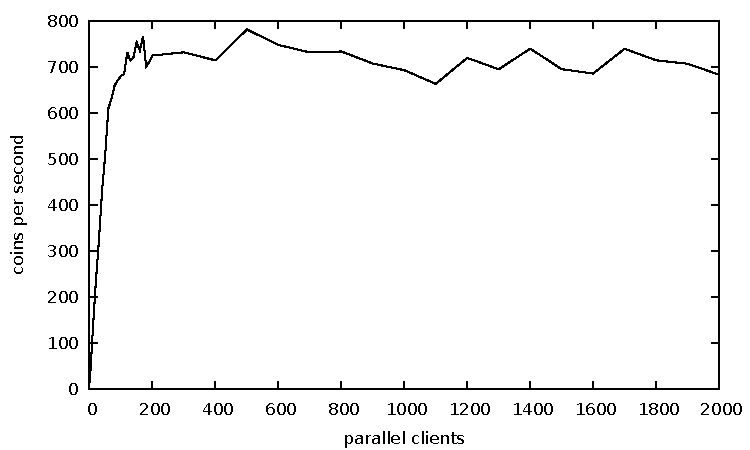
\includegraphics[width=\textwidth]{plots/speed.pdf}
  \caption[Coin throughput.]{Coin throughput in relation to number of parallel clients, with $1000$ coins per client per experiment run.}
  \label{fig:benchmark-throughput}
\end{figure}

\begin{figure}
  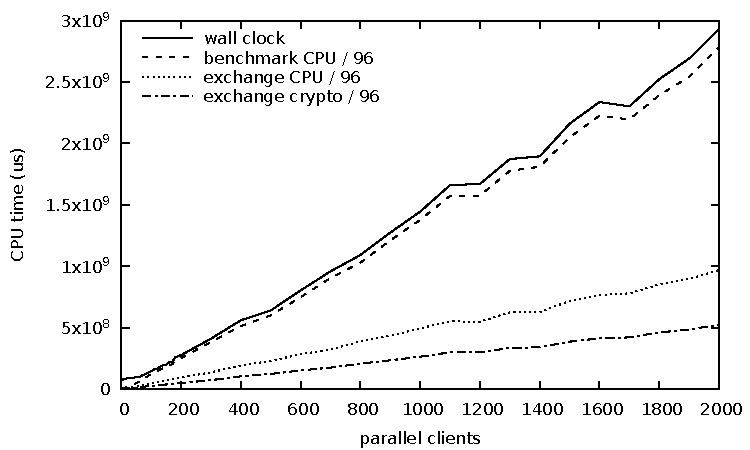
\includegraphics[width=\textwidth]{plots/cpu.pdf}
  \caption[Comparison of components' CPU usage for the benchmark.]{Comparison of real time, the CPU time for the exchange and the whole benchmark.}
  \label{fig:benchmark-cpu}
\end{figure}

\subsection{Latency}
We connected \texttt{firefly} and \texttt{gv} directly with a patch cable, and
introduced artificial network latency by configuring the Linux packet scheduler
with the \texttt{tc} tool.  The goal of this experiment was to observe the
network latency characteristics of the implementation.  Note that we do not consider
the overhead of TLS in our experiments, as we assume that TLS traffic is
already terminated before it reaches the exchange service, and exchanges can be
operated securely even without TLS.

The comparison between no additional delay and a \SI{100}{\milli\second} delay
is shown in Table~\ref{table:latency}.  TCP Fast Open~\cite{rfc7413} was
enabled on both \texttt{gv} and \texttt{firefly}.  Since for all operations
except \texttt{/refresh/reveal}, both request and response fit into one TCP
segment, these operations complete within one round-trip time.  This explains the
additional delay of $\approx \SI{200}{\milli\second}$ when the artificial delay
is introduced.  Without TCP Fast Open, we would observe an extra round trip for
the SYN and SYN/ACK packages without any payload.  The \texttt{/refresh/reveal}
operation takes an extra roundtrip due to the relatively large size of the
request (as show in Table~\ref{table:api-size}), which exceeds the MTU of 1500
for the link between \texttt{gv} and \texttt{firefly}, and thus does not fit
into the first TCP Fast Open packet.

Figure~\ref{fig:latencies} shows the latency for the exchange's HTTP endpoints
in relation to different network delays.  As expected, the additional delay
grows linearly for a single client.  We note that in larger benchmarks with
multiple parallel clients, the effect of additional delay would likely not just
be linear, due to timeouts raised by clients.

\newcommand{\specialcell}[2][c]{%
  \begin{tabular}[#1]{@{}c@{}}#2\end{tabular}}

\begin{table}
  \centering
  \begin{tabular}{lSSSS}
  \toprule
    Endpoint &
    {\specialcell[c]{Base latency\\(\si{\milli\second})}} &
    {\specialcell[c]{Latency with\\\SI{100}{\milli\second} delay\\(\si{\milli\second})}} \\
  \midrule
    \texttt{/keys}                &  1.14   &    201.25   \\ 
    \texttt{/reserve/withdraw}    &  22.68  &    222.46   \\ 
    \texttt{/deposit}             &  22.36  &   223.22    \\
    \texttt{/refresh/melt}        &  20.71  &    223.9    \\ 
    \texttt{/refresh/reveal}      &  63.64  &   466.30    \\
  \bottomrule
  \end{tabular}
  \caption{Effects of \SI{100}{\milli\second} symmetric network delay on total latency.}
  \label{table:latency}
\end{table}

\begin{table}
  \centering
  \begin{tabular}{lSSSS}
  \toprule
    Endpoint &
    {\specialcell[c]{Request size\\2048-bit RSA\\(\si{\kilo\byte})}} &
    {\specialcell[c]{Response size\\2048-bit RSA\\(\si{\kilo\byte})}} &
    {\specialcell[c]{Request size\\1024-bit RSA\\(\si{\kilo\byte})}} &
    {\specialcell[c]{Response size\\1024-bit RSA\\(\si{\kilo\byte})}} \\
  \midrule
    \texttt{/keys}                 & 0.14  & 3.75 & 0.14 & 3.43  \\ 
    \texttt{/reserve/withdraw}     & 0.73   & 0.71 & 0.60 & 0.49 \\ 
    \texttt{/deposit}              & 1.40   & 0.34 & 1.14 & 0.24  \\
    \texttt{/refresh/melt}         & 1.06   & 0.35 & 0.85 & 0.35  \\ 
    \texttt{/refresh/reveal}       & 1.67   & 2.11 & 1.16 & 1.23 \\
  \bottomrule
  \end{tabular}
  \caption[Request and response sizes for the exchange's API.]{Request and response sizes for the exchange's API.
  In addition to the sizes for 2048-bit RSA keys (used throughout the benchmark), the sizes for 1024-bit RSA keys are also provided.}
  \label{table:api-size}
\end{table}

\begin{figure}
  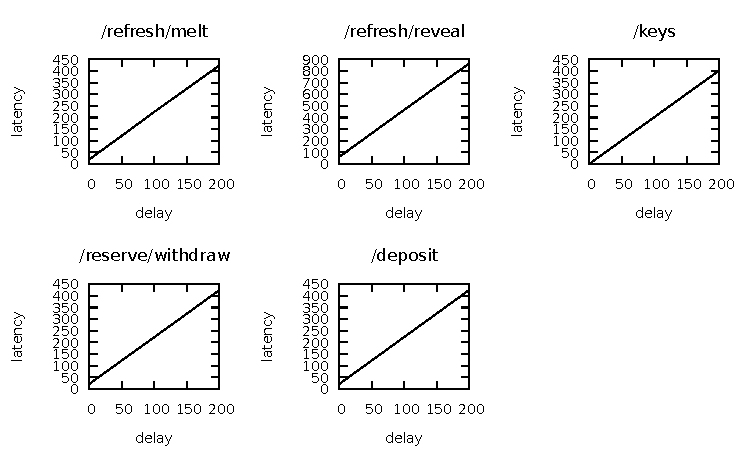
\includegraphics[width=\textwidth]{plots/latencies.pdf}
  \caption[Effect of artificial network delay on exchange's latency.]{Effect of artificial network delay on exchange's latency.}
  \label{fig:latencies}
\end{figure}

% Missing benchmarks:
% overall Taler tx/s
% db io+tx/s
% If I have time:
% traffic/storage depending on key size?


\section{Current Limitations and Future Improvements}\label{sec:implementation-improvements}
Currently the auditor does not support taking samples of deposit confirmations that
merchants receive.  The API and user interface to receive and process proofs
of misbehavior of the exchange/merchant generated by the wallet is not implemented yet.

As a real-world deployment of electronic cash has rather high requirements for
the operational security, the usage of hardware security modules for generation
of signatures should be considered.  Currently, a single process has access to
all key material.  For a lower-cost improvement that decreases the performance
of the system, a threshold signature scheme could be used.

The current implementation is focused on web payments.  To use GNU Taler for
payments in brick-and-mortar stores, hardware wallets and smartphone apps for
devices with near-field-communication (NFC) must be developed.  In some
scenarios, either the customer or the merchant might not have an Internet
connection, and this must be considered in the protocol design.  In typical
western brick-and-mortar stores, it is currently more likely that the merchant
has Internet connectivity, and thus the protocol must allow operations of the
wallet (such as refreshing) to be securely routed over the merchant's
connection.  In other scenarios, typically in developing countries, the
merchant (for example, a street vendor) might not have Internet connection.  If
the vendor has a smartphone, the connection to the merchant can be routed
through the customer.  In other cases, street vendors only have a ``dumb
phone'' that can receive text messages, and the payment goes through a provider
trusted by the merchant that sends text messages as confirmation for payments.
All these possibilities must be considered both from the perspective of the procotol and APIs
as well as the user experience.

% FIXME: explain that exchange does threading

Our experiments were only done with single exchange process and a single
database on the same machine.  There are various ways to horizontally scale the
exchange:
\begin{itemize}
  \item Multiple exchange processes can be run on multiple machines and access
    the database that runs a separate machine.  Requests are directed to the
    machines running the exchange process via a load balancer.  In this
    scenario, the throughput of the database is likely to be the bottleneck.
  \item To avoid having the database as a bottleneck, the contents can be
    partitioned into shards.  For this technique to be effective, data in the
    shards should not have any dependencies in other shards. A natural way to
    do sharding for the Taler exchange is to give each shard the sole
    responsibility for a subset of all available denominations.
  \item If the transaction volume on one denomination is too high to handle for
    a single shard, transactions can be further partitioned based on the coin's
    public key.  Each would maintain the database of spent/refreshed coins for
    a subset of all possible coin public keys.  This approach has been
    suggested for a centrally-banked cryprocurrency by Danezis and Meiklejohn
    \cite{danezis2016rscoin}.
\end{itemize}

% paranoid wallet (permissions!)

% FIXME: I want to mention PADs for auditing/transparency somewhere, just
% because they're cool


% FIXME:  coin locking not implemented!
